% Soubory musí být v kódování, které je nastaveno v příkazu \usepackage[...]{inputenc}
\PassOptionsToPackage{table, xcdraw}{xcolor}

\documentclass[%        Základní nastavení
%  draft,    				  % Testovací překlad
  12pt,       				% Velikost základního písma je 12 bodů
  a4paper,    				% Formát papíru je A4
  oneside,      			% Jednostranný tisk
	%twoside,      			% Dvoustranný tisk (kapitoly a další důležité části tedy začínají na lichých stranách)
	unicode,						% Záložky a metainformace ve výsledném  PDF budou v kódování unicode
]{report}				    	% Dokument třídy 'zpráva', vhodná pro sazbu závěrečných prací s kapitolami

\usepackage[utf8]		  %	Kódování zdrojových souborů je UTF-8
	{inputenc}					% Balíček pro nastavení kódování zdrojových souborů

\usepackage[				% Nastavení geometrie stránky
	bindingoffset=10mm,		% Hřbet pro vazbu
	hmargin={25mm,25mm},	% Vnitřní a vnější okraj
	vmargin={25mm,34mm},	% Horní a dolní okraj
	footskip=17mm,			  % Velikost zápatí
	nohead,					      % Bez záhlaví
	marginparsep=2mm,		  % Vzdálenost marginálií
	marginparwidth=18mm,	% Šířka marginálií
]{geometry}

\usepackage{sectsty}
	%přetypuje nadpisy všech úrovní na bezpatkové, kromě \chapter, která je přenastavena zvlášť v thesis.sty
	\allsectionsfont{\sffamily}

\usepackage{graphicx} % Balíček 'graphicx' pro vkládání obrázků
											% Nutné pro vložení logotypů školy a fakulty

\usepackage[          % Balíček 'acronym' pro sazby zkratek a symbolů
	nohyperlinks				% Nebudou tvořeny hypertextové odkazy do seznamu zkratek
]{acronym}						
											% Nutné pro použití prostředí 'acronym' balíčku 'thesis'

\usepackage[
	breaklinks=true,		% Hypertextové odkazy mohou obsahovat zalomení řádku
	hypertexnames=false % Názvy hypertext. odkazů budou tvořeny nezávisle na názvech TeXu
]{hyperref}						% Balíček 'hyperref' pro sazbu hypertextových odkazů
											% Nutné pro použití příkazu 'pdfsettings' balíčku 'thesis'

\usepackage{pdfpages} % Balíček umožňující vkládat stránky z PDF souborů
                      % Nutné při vkládání titulních listů a zadání přímo
                      % ve formátu PDF z informačního systému

\usepackage{enumitem} % Balíček pro nastavení mezerování v odrážkách
  \setlist{topsep=0pt,partopsep=0pt,noitemsep} % konkrétní nastavení

\usepackage{cmap} 		% Balíček cmap zajišťuje, že PDF vytvořené `pdflatexem' je
											% plně "prohledávatelné" a "kopírovatelné"

%\usepackage{upgreek}	% Balíček pro sazbu stojatých řeckých písmem
											%% např. stojaté pí: \uppi
											%% např. stojaté mí: \upmu (použitelné třeba v mikrometrech)
											%% pozor, grafická nekompatibilita s fonty typu Computer Modern!
                      
%\usepackage{amsmath} %balíček pro sabu náročnější matematiky                 

\usepackage{dirtree}	% sazba adresářové struktury
                      % vhodné pro prezentaci obsahu elektronické přílohy (např. CD)

\usepackage[formats]{listings}	% Balíček pro sazbu zdrojových textů
\lstset{              % nastavení
%	Definice jazyka použitého ve výpisech
%    language=[LaTeX]{TeX},	% LaTeX
%	language={Matlab},		% Matlab
	language={C},           % jazyk C
    basicstyle=\ttfamily,	% definice základního stylu písma
    tabsize=2,			% definice velikosti tabulátoru
    inputencoding=utf8,         % pro soubory uložené v kódování UTF-8
		columns=fixed,  %fixed nebo flexible,
		fontadjust=true %licovani sloupcu
    extendedchars=true,
    literate=%  definice symbolů s diakritikou
    {á}{{\'a}}1
    {č}{{\v{c}}}1
    {ď}{{\v{d}}}1
    {é}{{\'e}}1
    {ě}{{\v{e}}}1
    {í}{{\'i}}1
    {ň}{{\v{n}}}1
    {ó}{{\'o}}1
    {ř}{{\v{r}}}1
    {š}{{\v{s}}}1
    {ť}{{\v{t}}}1
    {ú}{{\'u}}1
    {ů}{{\r{u}}}1
    {ý}{{\'y}}1
    {ž}{{\v{z}}}1
    {Á}{{\'A}}1
    {Č}{{\v{C}}}1
    {Ď}{{\v{D}}}1
    {É}{{\'E}}1
    {Ě}{{\v{E}}}1
    {Í}{{\'I}}1
    {Ň}{{\v{N}}}1
    {Ó}{{\'O}}1
    {Ř}{{\v{R}}}1
    {Š}{{\v{S}}}1
    {Ť}{{\v{T}}}1
    {Ú}{{\'U}}1
    {Ů}{{\r{U}}}1
    {Ý}{{\'Y}}1
    {Ž}{{\v{Z}}}1
}

\usepackage{hyperref}

%%%%%%%%%%%%%%%%%%%%%%%%%%%%%%%%%%%%%%%%%%%%%%%%%%%%%%%%%%%%%%%%%
%%%%%%      Definice informací o dokumentu             %%%%%%%%%%
%%%%%%%%%%%%%%%%%%%%%%%%%%%%%%%%%%%%%%%%%%%%%%%%%%%%%%%%%%%%%%%%%

% V tomto souboru se nastavují téměř veškeré informace, proměnné mezi studenty:
% jméno, název práce, pohlaví atd.
% Tento soubor je SDÍLENÝ mezi textem práce a prezentací k obhajobě -- netřeba něco nastavovat na dvou místech.

\usepackage[
%%% Z následujících voleb jazyka lze použít pouze jednu
  czech-english,		% originální jazyk je čeština, překlad je anglicky (výchozí)
  %english-czech,	% originální jazyk je angličtina, překlad je česky
  %slovak-english,	% originální jazyk je slovenština, překlad je anglicky
  %english-slovak,	% originální jazyk je angličtina, překlad je slovensky
%
%%% Z následujících voleb typu práce lze použít pouze jednu
  semestral,		  % semestrální práce (nesází se abstrakty, prohlášení, poděkování) (výchozí)
  %bachelor,			%	bakalářská práce
  %master,			  % diplomová práce
  %treatise,			% pojednání o dizertační práci
  %doctoral,			% dizertační práce
%
%%% Z následujících voleb zarovnání objektů lze použít pouze jednu
%  left,				  % rovnice a popisky plovoucích objektů budou zarovnány vlevo
	center,			    % rovnice a popisky plovoucích objektů budou zarovnány na střed (vychozi)
%
]{thesis}   % Balíček pro sazbu studentských prací


%%% Jméno a příjmení autora ve tvaru
%  [tituly před jménem]{Křestní}{Příjmení}[tituly za jménem]
% Pokud osoba nemá titul před/za jménem, smažte celý řetězec '[...]'
\author[Bc.]{Křestní}{Příjmení}

%%% Pohlaví autora/autorky
% (nepoužije se ve variantě english-czech ani english-slovak)
% Číselná hodnota: 1...žena, 0...muž
\gender{0}

%%% Jméno a příjmení vedoucího/školitele včetně titulů
%  [tituly před jménem]{Křestní}{Příjmení}[tituly za jménem]
% Pokud osoba nemá titul před/za jménem, smažte celý řetězec '[...]'
\advisor[prof.\ Ing.]{Křestní}{Příjmení}[CSc.]

%%% Jméno a příjmení oponenta včetně titulů
%  [tituly před jménem]{Křestní}{Příjmení}[tituly za jménem]
% Pokud osoba nemá titul před/za jménem, smažte celý řetězec '[...]'
% Nastavení oponenta se uplatní pouze v prezentaci k obhajobě;
% v případě, že nechcete, aby se na titulním snímku prezentace zobrazoval oponent, pouze příkaz zakomentujte;
% u obhajoby semestrální práce se oponent nezobrazuje (jelikož neexistuje)
\opponent[doc.\ Mgr.]{Křestní}{Příjmení}[Ph.D.]

%%% Název práce
%  Parametr ve složených závorkách {} je název v originálním jazyce,
%  parametr v hranatých závorkách [] je překlad (podle toho jaký je originální jazyk)
\title[Title of Student's Thesis]{Název studentské práce}

%%% Označení oboru studia
%  Parametr ve složených závorkách {} je název oboru v originálním jazyce,
%  parametr v hranatých závorkách [] je překlad
\specialization[Teleinformatics]{Teleinformatika}

%%% Označení ústavu
%  Parametr ve složených závorkách {} je název ústavu v originálním jazyce,
%  parametr v hranatých závorkách [] je překlad
%\department[Department of Control and Instrumentation]{Ústav automatizace a měřicí techniky}
%\department[Department of Biomedical Engineering]{Ústav biomedicínského inženýrství}
%\department[Department of Electrical Power Engineering]{Ústav elektroenergetiky}
%\department[Department of Electrical and Electronic Technology]{Ústav elektrotechnologie}
%\department[Department of Physics]{Ústav fyziky}
%\department[Department of Foreign Languages]{Ústav jazyků}
%\department[Department of Mathematics]{Ústav matematiky}
%\department[Department of Microelectronics]{Ústav mikroelektroniky}
%\department[Department of Radio Electronics]{Ústav radioelektroniky}
%\department[Department of Theoretical and Experimental Electrical Engineering]{Ústav teoretické a experimentální elektrotechniky}
\department[Department of Telecommunications]{Ústav telekomunikací}
%\department[Department of Power Electrical and Electronic Engineering]{Ústav výkonové elektrotechniky a elektroniky}

%%% Označení fakulty
%  Parametr ve složených závorkách {} je název fakulty v originálním jazyce,
%  parametr v hranatých závorkách [] je překlad
%\faculty[Faculty of Architecture]{Fakulta architektury}
\faculty[Faculty of Electrical Engineering and~Communication]{Fakulta elektrotechniky a~komunikačních technologií}
%\faculty[Faculty of Chemistry]{Fakulta chemická}
%\faculty[Faculty of Information Technology]{Fakulta informačních technologií}
%\faculty[Faculty of Business and Management]{Fakulta podnikatelská}
%\faculty[Faculty of Civil Engineering]{Fakulta stavební}
%\faculty[Faculty of Mechanical Engineering]{Fakulta strojního inženýrství}
%\faculty[Faculty of Fine Arts]{Fakulta výtvarných umění}
%
%Nastavení logotypu (v hranatych zavorkach zkracene logo, ve slozenych plne):
\facultylogo[logo/FEKT_zkratka_barevne_PANTONE_CZ]{logo/UTKO_color_PANTONE_CZ}

%%% Rok sepsání práce
\graduateyear{2030}

%%% Datum obhajoby (uplatní se pouze v prezentaci k obhajobě)
\date{11.\,11.\,1980} 

%%% Místo obhajoby
% Na titulních stránkách bude automaticky vysázeno VELKÝMI písmeny (pokud tyto stránky sází šablona)
\city{Brno}

%%% Abstrakt
\abstract[%
Překlad abstraktu
(v~angličtině, pokud je originálním jazykem čeština či slovenština; v~češtině či slovenštině, pokud je originálním jazykem angličtina)
]{%
Abstrakt práce v~originálním jazyce
}

%%% Klíčová slova
\keywrds[%
Překlad klíčových slov
(v~angličtině, pokud je originálním jazykem čeština či slovenština; v~češtině či slovenštině, pokud je originálním jazykem angličtina)
]{%
Klíčová slova v~originálním jazyce
}

%%% Poděkování
\acknowledgement{%
Rád bych poděkoval vedoucímu diplomové práce panu Ing.~XXX YYY, Ph.D.\ za odborné vedení, konzultace, trpělivost a podnětné návrhy k~práci.
}%  % do tohoto souboru doplňte údaje o sobě, druhu práce, názvu...

%%%%%%%%%%%%%%%%%%%%%%%%%%%%%%%%%%%%%%%%%%%%%%%%%%%%%%%%%%%%%%%%%%%%%%%%

%%%%%%%%%%%%%%%%%%%%%%%%%%%%%%%%%%%%%%%%%%%%%%%%%%%%%%%%%%%%%%%%%%%%%%%%
%%%%%%     Nastavení polí ve Vlastnostech dokumentu PDF      %%%%%%%%%%%
%%%%%%%%%%%%%%%%%%%%%%%%%%%%%%%%%%%%%%%%%%%%%%%%%%%%%%%%%%%%%%%%%%%%%%%%
%% Při načteném balíčku 'hyperref' lze použít příkaz '\pdfsettings':
\pdfsettings
%  Nastavení polí je možné provést také ručně příkazem:
%\hypersetup{
%  pdftitle={Název studentské práce},    	% Pole 'Document Title'
%  pdfauthor={Autor studenstké práce},   	% Pole 'Author'
%  pdfsubject={Typ práce}, 						  	% Pole 'Subject'
%  pdfkeywords={Klíčová slova}           	% Pole 'Keywords'
%}
%%%%%%%%%%%%%%%%%%%%%%%%%%%%%%%%%%%%%%%%%%%%%%%%%%%%%%%%%%%%%%%%%%%%%%%

\pdfmapfile{=vafle.map}

%%%%%%%%%%%%%%%%%%%%%%%%%%%%%%%%%%%%%%%%%%%%%%%%%%%%%%%%%%%%%%%%%%%%%%%
%%%%%%%%%%%       Začátek dokumentu               %%%%%%%%%%%%%%%%%%%%%
%%%%%%%%%%%%%%%%%%%%%%%%%%%%%%%%%%%%%%%%%%%%%%%%%%%%%%%%%%%%%%%%%%%%%%%
\begin{document}
\pagestyle{empty} %vypnutí číslování stránek

%% Vložení desek 
\includepdf[pages=1]%  buďto generovaných informačním systémem
  {pdf/desky}% název souboru nesmí obsahovat mezery!
%% NEBO vytvoření desek z balíčku
%\makecover
%%
\oddpage % při dvojstranném tisku přidá prázdnou stránku
% kazdopádně ale:
\setcounter{page}{1} %resetovaní čítače stránek -- desky do číslování nezahrnujeme

%% Vložení titulního listu
\includepdf[pages=1]%    buďto generovaného informačním systémem
  {pdf/titulka}% název souboru nesmí obsahovat mezery!
%% NEBO vytvoření titulní stránky z balíčku
%\maketitle
%%
\oddpage  % při dvojstranném tisku se přidá prázdná stránka
   
%% Vložení zadání
\includepdf[pages=1]%   buďto generovaného informačním systémem
  {pdf/zadani}% název souboru nesmí obsahovat mezery!
%% NEBO lze vytvořit prázdný list příkazem ze šablony
%\patternpage{}%
%	{\sffamily\Huge\centering ZDE VLOŽIT LIST ZADÁNÍ}%
%	{\sffamily\centering Z~důvodu správného číslování stránek}
%%
\oddpage% při dvojstranném tisku se přidá prázdná stránka

%% Vysázení stránky s abstraktem
\makeabstract

% Vysázení stránky s rozšířeným abstraktem
% (pokud píšete práci v češtině či slovenštině, vložení rozšířeného abstraktu zrušte;
%  pro semestrální projekt také není potřeba rozšířený abstrakt uvádět)
%% Vysázení stránky s rozšířeným abstraktem
% (týká se pouze bc. a dp. prací psaných v angličtině, viz Směrnice rektora 72/2017)
\cleardoublepage
\noindent
{\large\sffamily\bfseries\MakeUppercase{Rozšířený abstrakt}}
\\
Výtah ze směrnice rektora 72/2017:\\
\emph{Bakalářská a diplomová práce předložená v angličtině musí obsahovat rozšířený abstrakt v češtině
nebo slovenštině (čl. 15). To se netýká studentů, kteří studují studijní program akreditovaný v
angličtině.}
(čl. 3, par. 7)\\
\emph{Nebude-li vnitřní normou stanoveno jinak, doporučuje se rozšířený abstrakt o rozsahu přibližně 3
normostrany, který bude obsahovat úvod, popis řešení a shrnutí a zhodnocení výsledků.}
(čl. 15, par. 5)

%%% Vysázení citace práce
\makecitation

%%% Vysázení prohlášení o samostatnosti
\makedeclaration

%%% Vysázení poděkování
\makeacknowledgement

%%% Vysázení obsahu
\tableofcontents

\cleardoublepage\pagestyle{plain}   % zapnutí číslování stránek

%Pro vkládání kapitol i příloh používejte raději \include než \input
%%% Vložení souboru 'text/uvod.tex' s úvodem
\chapter*{Úvod}
\phantomsection
\addcontentsline{toc}{chapter}{Úvod}

Tato práce se zabývá návrhem elektronické hry Logic. Tato hra by se měla co nejvíce podobat deskové hře a~musí respektovat pravidla deskové 
hry. Hra Logic je určená pro všechny věkové kategorie hráčů. Podporuje a~rozvíjí logické myšlení. 

Hra musí být navržena jako přenosné zařízení, takže musí být kladen důraz na spotřebu jednotlivých použitých komponentů.

Hra Logic není komerčně dostupná v~elektronické verzi. Existuje pouze ve verzi deskové hry pro dva hráče. Elektronická hra Logic je 
navržena pro jednoho hráče. Hra je jedinečná svými ovládacími prvky a~způsobem hry. 

V~této práci je popsán návrh elektronické hry. Na začátku jsou popsána pravidla deskové hry, která jsou respektována i~u~elektronické hry. 
Elektronická hra Logic je tvořena DPS, která obsahuje veškeré potřebné komponenty pro funkci hry i~pro její ovládání.

Na závěr je popsán způsob elektronické hry a~její ovládání.


%Šablona je nastavena na \emph{dvoustranný tisk}. Pokud máte nějaký závažný důvod sázet (a~zejména tisknout) jednostranně, nezapomeňte si přepnout volbu \texttt{twoside} na \texttt{oneside}!

%%% Vložení souboru 'text/reseni' s popisem řešení práce
% (rozdělte na více souborů či kapitol, pokud je vhodné)
\chapter{Pravidla hry}
Logic je desková hra pro dva hráče. Jeden hráč určí hledanou kombinaci, dále bude označován jako hráč A, a druhý tuto kombinaci za pomocí logických úvah a
vyhodnocení hráčem A hledá, dále bude označován jako hráč B.

Hráči si určí herní pozice. Hráč A vybere barvy a následně je v určitém pořadí vloží do zadávacího pole a zakryje je, aby tuto
kombinaci spoluhráč neviděl. Hráč B je v této chvíli otočen. Hráč B následně zvolí náhodnou kombinaci barev a pozic. Po ukončení tahu nechá
hráče A, aby tah vyhodnotil. Hráč A vyhodnotí tah následujícím způsobem. Pokud hráč B vložil správnou barvu na správnou pozici, tak vloží 
do vyhodnocovací sekce černý kolík. Pokud vložil barvu, která se v zadání vyskytuje, ale vložil ji na nesprávnou pozici, tak vloží bílý kolík.
Pokud zůstanou některé pozice neobsazené, tak to znamená, že daná barva se v zadání nevyskytuje. Poté začne hráč B na základě vyhodnocení a 
svých všech předchozích tahů hledat kombinaci.

Cílem hry je nalézt správnou kombinaci dříve, než skončí plocha herního pole.

Těžší varianta spočívá v možnosti absence barvy - v zadání je mezera.

\chapter{Popis zapojení}

\section{Procesor}
Byl vybrán procesor ESP32-PICO-D4.

Tento procesor obsahuje \cite{PICO_datasheet}: %napsáno zatím pro WROOM - opravit
\begin{itemize}
    \item WiFi,
    \item Bluetooth,
    \item procesor,
    \item průměrný odběr proudu 80 mA,
    \item 32 GPIO pinů,
    \item dvoujádrový 32bitový procesor Xtensa LX6,
    \item 520 kB SRAM, %?
    \item 16 MB FLASH. %?
  \end{itemize}

  Napájecí napětí tohoto procesoru je od 3,0 do 3,6 V \cite{PICO_datasheet}. ESP32-PICO má vyvedeno 32 GPIO pinů, které je 
  možno softwarově nastavit jako vstupní nebo výstupní. Na tyto piny lze poté připojit různá zařízení. Vstupním senzorem může 
  být typicky tlačítko a výstupním indikátorem např. LED. Tato zařízení zprostředkovávají komunikaci mezi procesorem a okolním 
  světem.

  Zapojení pinu EN bylo převzato ze schématu \cite{PICO_datasheet}.

  GPIO piny IO16 a IO17 nemohou být použity, protože ESP32-PICO má na těchto pinech připojenou flash paměť \cite{PICO_datasheet}.
  Pokud by na tento pin bylo něco připojeno, tak by se procesor nedostal do své paměti. Nahraný program do procesoru by tedy
  nemohl být načten a DPS by ztratila svoji funkci.

  GPIO piny IO34 a vyšší jsou pouze vstupní \cite{PICO_datasheet}. Vstupní piny nemají softwarově zapojitelný pullup rezistor. 
  Pokud je tedy zapotřebí pullup rezistor, musí se fyzicky zapojit.
  
  \section{Napájení}
  \subsection{v0.0}
  \subsection{v1.0}
  Ve verzi 1.0 bylo napájení předěláno. Napájení v této verzi neprobíhá přes baterie, ale pouze přes USB konektor. Byl 
  zvolen konektor USB Micro.
  Výhody:
  \begin{itemize}
    \item Absence nabíjecího obvodu,
    \item absence hlídání stavu nabití baterie,
    \item absence ochrany proti přepólování (USB konektor je uzpůsoben svým tvarem, aby uživatel nemohl napájení přepólovat.),
    \item .
  \end{itemize}

  Nevýhody:
  \begin{itemize}
    \item Předpokládá se, že uživatel vlastní powerbanku.% vymyslet další
  \end{itemize}

  \section{Stepdown}
  Procesor ESP32-PICO-D4 má napájecí napětí 3,3 V. Napětí z powerbanky přes USB je 5 V. Proto je tedy zapotřebí zapojit 
  stepdown, který bude vytvářet napájecí napětí pro procesor.

  Jako stepdown byl zvolen čip SY8105.
  Parametry čipu SY8105 \cite{SY8105_datasheet}:
  \begin{itemize}
    \item Vstupní napětí 1,5 - 18 V,
    \item výstupní proud 5 A,
    \item pouzdro TSOT23-6.
  \end{itemize}

  \begin{figure}[!h]
    \begin{center}
      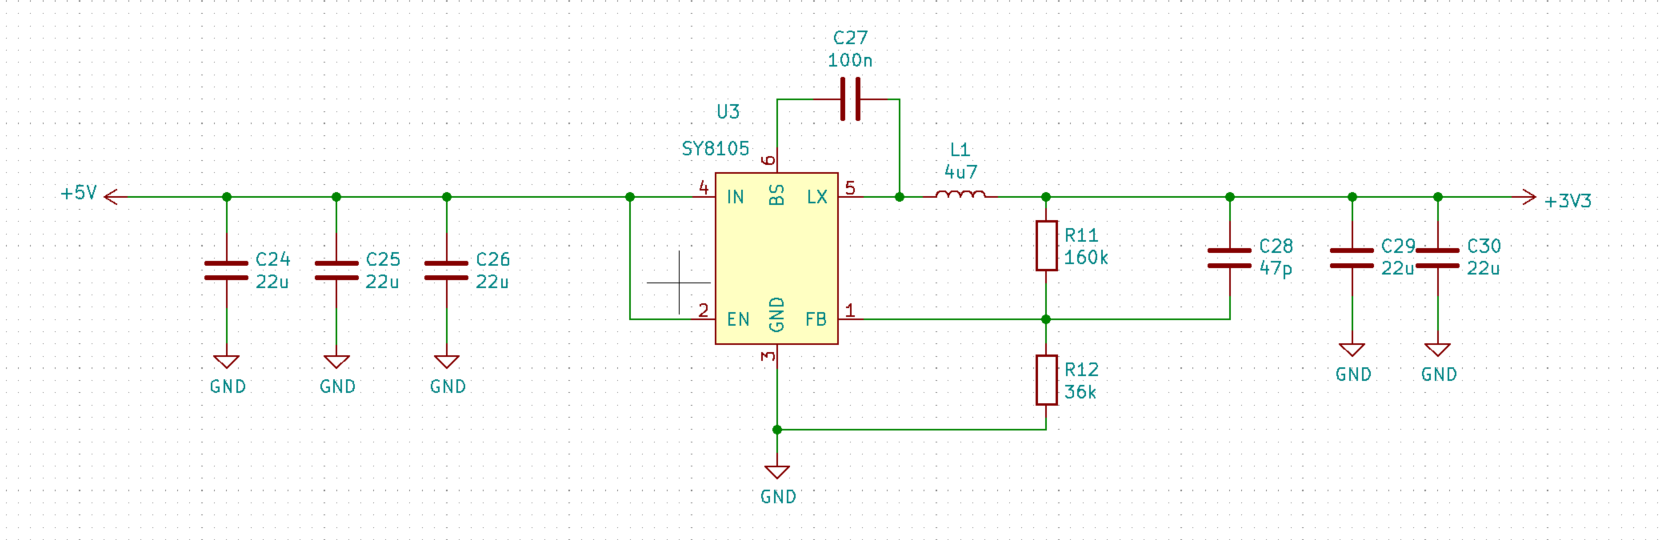
\includegraphics[scale=0.5]{obrazky/SY8105_schema.png}
    \end{center}
    \caption[SY8105 schéma]{Schéma zapojení čipu SY8105 \cite{SY8105_datasheet}.}
  \end{figure}

  Výstupní napětí je závislé na poměru odporů R11 a R12. Nastavené velikosti odporů jsou pro výstupní napětí 3,3 V pro procesor 
  ESP32-PICO.

  \section{Převodník z USB na RS-232}
  Procesor ESP32-PICO používá jako komunikační rozhraní linku RS-232. Programování ale probíhá přes USB, které toto rozhraní
  nemá. Proto bylo potřeba použít převodník z USB na rozhraní RS-232.
  
  Pro převod z USB na RS-232 byl použit čip CP2102, který  zároveň převádí logiku 0 - 5 V na logiku 0 - 3,3 V 
  \cite{CP2102_datasheet}.%protože je i na devkitu

Parametry čipu CP2102 [citace]:
\begin{itemize}
    \item 
\end{itemize}

\begin{figure}[!h]
    \begin{center}
      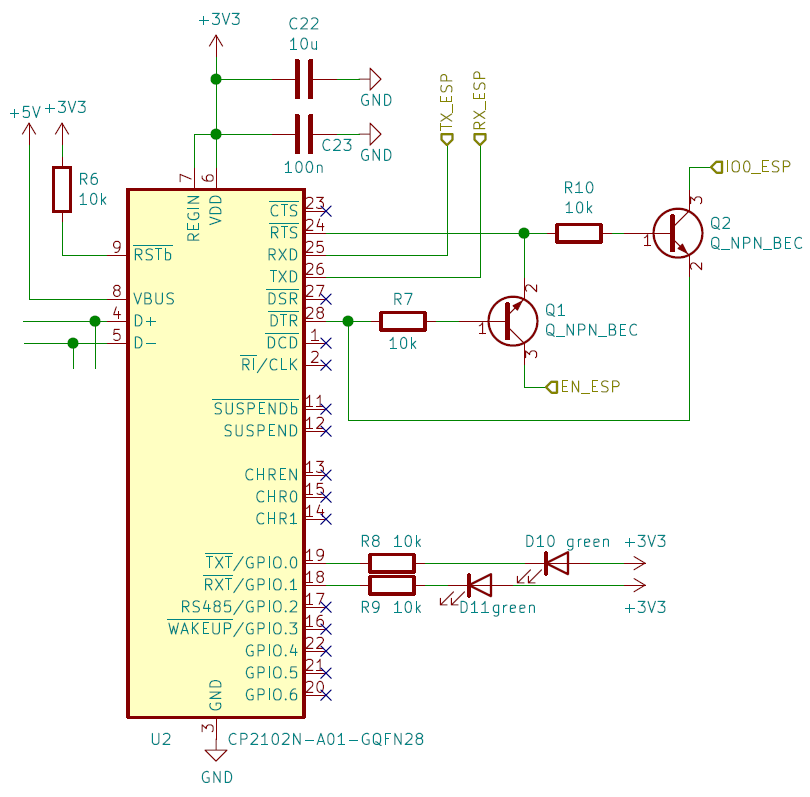
\includegraphics[scale=0.5]{obrazky/CP2102_schema.png}
    \end{center}
    \caption[CP2102 schéma]{Schéma zapojení převodníku z USB na RS-232 [citace asi devkit].}
\end{figure}

Z USB jsou signály D+ a D- připojeny k čipu CP2102. Tento čip tento signál převede na signály RX a TX, které mají výstup 
na pinech RXD a TXD. Následně jsou tyto signály připojeny k procesoru ESP32-PICO. Signály RX a TX se musí překřížit – RX 
CP2102 se připojí na TX ESP32-PICO a TX CP2102 se připojí na RX ESP32-PICO. 

LED D10 a D11 slouží k indikaci komunikace s procesorem. Jsou zapojeny podle datasheetu \cite{CP2102_datasheet}. Pokud je do 
procesoru nahráván program, tak LED D10 a D11 blikají.

\begin{figure}[!h]
    \begin{center}
      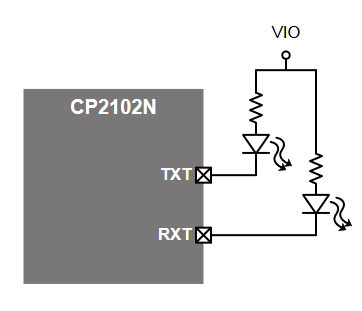
\includegraphics[scale=0.5]{obrazky/CP2102_LED.png}
    \end{center}
    \caption[CP2102 LED]{Zapojení LED pro indikaci komunikace s procesorem k čipu CP2102 \cite{CP2102_datasheet}.}
\end{figure}

\section{LED}
Byly vybrány LED typu WS2812C. Tento typ LED je určen pro přenosná zařízení, díky jejich nízké spotřebě. Každá LED 
má v sobě procesor, který slouží pro zpracování dat. LED přebírají informaci o barvě v RGB formátu. 
Tyto LED byly vybrány z důvodu nízké spotřeby a také kvůli jednoduchému přístupu z pohledu programování.
LED WS2812C se zapojují za sebou přes piny DATA OUT a DATA IN. Každá LED si přebere data, která jsou pro ni a zbytek pošle 
další LED.

Parametry LED WS2812C [citace]: %přidat
\begin{itemize}
    \item 
\end{itemize}

Porovnání WS2812C s WS2812B:
%tabulka

Ke každé LED je připojen na napájení filtrační kondenzátor [citace na doporučení z datasheetu], aby LED svítili kontinuálně 
a nedostal se jim na napájení žádný šum.

\subsection{Rozdělení}
LED jsou rozděneny do tří skupin. Skupina LED pro zadání, skupina LED pro herní pole a skupina LED pro zobrazení vyhodnocení 
tahu.
Skupina LED pro zadání obsahuje 4 LED a skupiny pro herní pole a pro vyhodnocení každá 40 LED.

\section{Zapínání LED}
DPS je navrhována pro přenosnou aplikaci, a proto je potřeba zajistit její co nejnižší odběr. 

LED mají určitou spotřebu, i když zrvona nesvítí žádnou barvou. Proto je herní pole dohromady s vyhodnocovacími LED rozděleno 
na 3 části. Do první části patří LED se zadáním a první 4 čtveřice LED z herního pole a z vyhodnocení. Do druhé části patří 
další 3 čtveřice LED z herního pole a z vyhodnocení. Do třetí části patří poslední 3 čtveřice LED z herního pole a z 
vyhodnocení.

Těmto 3 částem je postupně zapínáno napájecí napětí. Každé části se zapne napájení až pokud se hráč dostane do fáze, kdy 
danou oblast bude potřebovat. K zapínání dochází softwarově spínáním GPIO pinem procesoru.

Ke spínání slouží obvody s MOSFET tranzistory. MOSFET tranzistory byly zvoleny pro jejich nulovou spotřebu, narozdíl od 
bipolárních tranzistorů. 
%přidat obrázek

\subsection{Popis funkce}
%přepsat

\section{Spínací prvky}
Přepínač SW1 slouží pro zapínání celé DPS. Tento přepínač připojuje napájecí napětí 5 V z USB k celému zbytku DPS.

Tlačítka slouží pro ovládání hry. Ke každému tlačítku je připojen kondenzátor o hodnotě 100 nF. Tento kondenzátor 
slouží pro filtraci zákmitů při zmáčknutí tlačítka. Filtrace se proto nemusí řešit softwarově.

\section{PowerLED}
Diody D1 a D2 slouží pro indikaci přítomnosti napájecího napětí.  Dioda D1 indikuje přítomnost napájecího napětí 
5 V a dioda D2 indikuje přítomnost napájecího napětí 3,3 V.

\chapter{Popis DPS}
DPS je navržena v programu KiCad a její parametry jsou určeny pro výrobu i osazení ve firmě JLCPCB \cite{JLCPCB}. Výrobní 
podklady proto musely být navrženy v souladu s jejich výrobními možnostmi \cite{JLCPCB_Capabilities}.

DPS má 4 vrstvy. Vnitřní vrstvy slouží pro napájení a vnější pro signálové dráhy. V jedné vnitřní vrstvě je po celé její ploše 
rozlité GND a ve druhé vnitřní vrstvě jsou rozlitá jednotlivá napájecí napětí.

Na vrchní straně jsou umístěny i plošky pro osazení SMD součástek, protože firma JLCPCB osazuje pouze SMD součástky z jedné 
strany. THT součástky jsou připraveny na ruční pájení.

Signálové dráhy jsou vedeny tenkou dráhou a napájecí dráhy jsou vedeny tlusčí dráhou. V signálových drahách tečou zanedbatelné 
proudy, proto mohou být co nejtenčí. Výrobce umožňuje vyrobit nejtenčí dráhu u čtyřvrstvé DPS 0,09 mm \cite{JLCPCB_Capabilities}. 
Aby nebyly použity krajní hodnoty, byla zvolena šířka signálové dráhy 0,150 mm.

Kondenzátoty u procesoru ESP32-PICO a u čipu CP2102 musí být umístěny co nejblíže jejich pouzdru. Tyto kondenzátory slouží pro 
filtraci šumu na napájení.

Dráhy od USB k čipu CP2102 D+ a D- fungují jako diferenciální pár. Proto musejí být jejich dráhy vedeny vedle sebe a blízko u 
sebe.

Rozložení počástek k čipu SY8105 na DPS může velmi ovlivnit jeho funkčnost. Rozložení a zapojení stepdownu 
bylo převzato z datasheetu \cite{SY8105_datasheet}. %vložit obrázek

LED jsou rozděleny do 3 skupin, aby se hra co nejvíce podobala deskové hře. LED pro zadání jsou v horní části DPS. V levém 
sloupci pod zadáním jsou LED, které slouží jako herní pole, a v pravém sloupci jsou LED pro vyhodnocení tahu.

\chapter{Oživení DPS}
DPS přijde z výroby ve stavu, kdy jsou osazeny pouze SMD komponenty. % fotka

Poté je nutné ručně osadit THT součástky, tj. vypínač, tlačítka a konektor USB micro. Připojení DPS přes USB k powerbance, 
nebo do počítače, se rozsvítí LED D1 a D2, které indikují přítomnost napájecího napětí. LED D2 zároveň značí, že stepdown je 
funkční.















%možná vůbec nebude, nebo bude určitě jinde
\section{Nabíjecí obvod}
Pro nabíjecí obvod byl zvolen čip TP4056. Jeho zapojení bylo převzato z datasheetu [citace]. %tady bude obrázek schématu asi
Velikost rezistoru $R_\textind{PROG}$ se volí podle nabíjecího proudu. 
Tabulka rezistorů $R_\textind{PROG}$.. [citace]

\begin{table}[!h]
    \caption{Nastavení nabíjecího proudu rezitorem $R_\textind{PROG}$}
    \begin{center}
        \begin{tabular}{|c|c|}
            \hline
            $R_\textind{PROG}$ [kOhm] & Nabíjecí proud [mA] \\
            \hline
            10      & 130 \\
            \hline
            5       & 250 \\
            \hline
            4       & 300 \\
            \hline
            3       & 400 \\
            \hline
            2       & 580 \\
            \hline
            1,66    & 690 \\
            \hline
            1,5     & 780 \\
            \hline
            1,33    & 900 \\
            \hline
            1,2     & 1000 \\
            \hline
        \end{tabular}
        
    \end{center}
\end{table}

Nabíjení baterií by mělo probíhat při 0,5C, tudíž pro 18650 je to cca 0,5 A. Proto byl zvolen rezitor Rprog 2 kOhm.


%%% Vložení souboru 'text/vysledky' s popisem vysledků práce
% (rozdělte na více souborů či kapitol, pokud je vhodné)
\chapter{Software}
Software pro Elektronickou hru Logic byl napsán v jazyce C++. Bylo využito skutečnosti, že mikrokontrolér ESP32-PICO podporuje Arduino 
framework. Pro psaní softwaru bylo použito vývojové prostředí Visual Studio Code. %kompilátor 

Pro programování inteligentních LED bylo využito již existující knihovny SmartLeds.h \cite{SmartLeds}.
Tato knihovna velmi usnadňuje softwarovou práci s těmito inteligentními LED. Obsahuje například funkci {\it show}, která umožní zobrazit 
nastavené barvy na všech inteligentních LED připojených k jednomu pinu mikrokontroléru ESP32-PICO. 

Celý software je rozdělen do dvou částí, počáteční inicializace a nekonečná smyčka programu. 

Po spuštění probíhá inicializace vstupně-výstupních pinů a teké inicializace proměnných. Všem inteligentním LED je vypnuto napájecí napětí. 
Dále je všem inteligentním LED nastavena barva na černou, tzn. LED nesvítí. Po kompletním nastavení se již čeká na stisk tlačítka "Nová hra". 

\section{Tlačítko Nová hra}
Když je stisknuto tlačítko "Nová hra", tak je všem inteligentním LED nastavena černá barva. Program načte stavy přepínačů. Pokud je nastavena hra pro 
jednoho hráče, tak je vygenerováno zadání. Pokud je hra s mezerou, tak je generace zadání rozšířena o černou barvu. Poslední přepínač určuje délku 
vygenerovaného zadání. V případě hry pro jednoho hráče je přepínač s mezerou ignorován. Následně je zapnuto napájecí napětí 
první části inteligentních LED a poté program přechází do druhé části, tj. nekonečné smyčky.

\begin{minipage}{\linewidth}
\begin{lstlisting}[frame=single,numbers=right,caption={Funkce pro vygenerování zadání.},label=lst:priklad.vypis.kodu.C,basicstyle=\ttfamily\small, keywordstyle=\color{black}\bfseries\underbar,]
void generate_task (Colors *task, int length, int diff){
    for(int i = 0; i < length; ++i)
        task[i] = Colors(esp_random() % (NUM_OF_COLORS - diff));
}     
void set_task(led_t &leds, Colors* array_task, int length){
    for (int i = 0; i < length; ++i){
        leds.pos = i;
        set_color(leds, array_task[i]); 
    } 
}   
\end{lstlisting}
\end{minipage} 

Nekonečná smyčka má dva hlavní úkoly. Detekuje stisknutí tlačítek a v pravidelných intervalech bliká kurzorem. Na konci každého průchodu smyčkou 
se obnoví zobrazení na inteligentních LED.

\section{Tlačítka interpretující šipky}
Po každém stisku některé z šipek program nejprve zjišťuje, zda je spuštěna hra pro jednoho, nebo pro dva hráče, a také, v případě hry pro dva
hráče, v jaké části inteligentních LED se právě nachází kurzor. Poté je kurzor dle dané šipky posunut buď o jedno pole vpravo, nebo o jedno 
pole vlevo, v rámci dané části inteligentních LED. 

Pokud se kurzor nachází na konci řádku a je stisknuto tlačítko "Šipka vpravo", je pozice přepočítána tak, aby se kurzor posunul na 
začátek téhož řádku. Pokud se kurzor nachází na začátku řádku a je stisknuto tlačítko "Šipka vlevo", je pozice přepočítána tak, aby se kurzor 
posunul na konec téhož řádku. 

\begin{minipage}{\linewidth}
\begin{lstlisting}[frame=single,numbers=right,caption={Funkce posouvající kurzor.},label=lst:priklad.vypis.kodu.C,basicstyle=\ttfamily\small, keywordstyle=\color{black}\bfseries\underbar,]
void shift_cursor (led_t &LED, Direct DIR, int length){
    if((DIR == RIGHT) && 
        !((LED.pos + 1 + LINE_LENGTH - length) % LINE_LENGTH))
        LED.pos -= LINE_LENGTH - (LINE_LENGTH - length) - 1;
    else if(DIR == RIGHT)
        LED.pos += 1;
    else if((DIR == LEFT) && 
            (LED.pos == 0 || !(LED.pos % LINE_LENGTH)))
        LED.pos += LINE_LENGTH - (LINE_LENGTH - length) - 1;
    else if(DIR == LEFT)
        LED.pos -= 1;
}   
\end{lstlisting}
\end{minipage} 
    
\section{Barevná tlačítka}
Po každém stisku barevného tlačítka program zjišťuje, zda je spuštěna hra pro jednoho, nebo pro dva hráče, a také, v případě hry pro dva hráče,
v jaké části inteligentních LED se právě nachází kurzor. Poté se nastaví v dané části daná barva LED na pozici kurzoru a kurzor se posune o 
jedno pole vpravo. Pokud se ve hře pro dva hráče nachází kurzor ve vyhodnocovací části, tak jsou stisky všech barev kromě červené a žluté 
ignorovány. Na konci průchodu smyčkou je tato změna zobrazena na inteligentních LED. 

\section{Tlačítko Potvrdit tah}
Po stisku tlačítka "Potvrdit tah"\  je zjištěno, zda je nastavena hra pro jednoho, nebo pro dva hráče. 

Pokud je nastavena hra pro jednoho hráče, tak dojde k vyhodnocení tahu a kurzor je posunut na první LED dalšího herního řádku. Pokud je již 
kurzor na posledním řádku, tak je zobrazeno zadání a kurzor přestává blikat. Pokud se shoduje herní kombinace se zadáním dříve, než na 
posledním řádku, tak je zobrazeno vyhodnocení i zadání. Kurzor přestává blikat a hra čeká na stisk tlačítka "Konec", nebo "Nová hra". 

Vyhodnocení probíhá ve dvou krocích. Nejdříve jsou hledány barvy na správných pozicích. Tyto barvy jsou ohodnoceny červeně. Pozice těchto 
barev jsou v dalších krocích vynechávány. Pokud je počet nalezených barev na shodných pozicích stejný, jako je délka zadání, tak vyhodnocení 
končí. Pokud tomu tak není, vyhodnocení pokračuje. Následně pokud je nalezena ve zbylých barvách barva, která je obsazena v zadání, tak je 
ohodnocena žlutou barvou. Každá ohodnocená barva se v dalších krocích již přeskakuje. 

Pokud je nastavena hra pro dva hráče, dojde k posunutí kurzoru na první LED části, která je právě na řadě. Pokud byl kurzor v zadání, posune
se do herního pole, pokud byl v herním poli, posune se do pole pro vyhodnocení a pokud byl kurzor v poli pro vyhodnocení, tak se přesune
do herního pole. 

Pokud má následující řádek vypnuto napájecí napětí, tak je toto napětí softwarově zapnuto. 

\section{Tlačítko Konec}
Pokud je stisknuto tlačítko "Konec", jsou všechny LED zhasnuty a poté je jim odpojeno napájecí napětí. Následně se čeká na stisk tlačítka
"Nová hra". 

\iffalse
\section{Funkce init}
Funkce {\it \_init\_} slouží pro inicializaci vstupně-výstupních pinů. Všechny piny, na kterých jsou připojena tlačítka, jsou nastaveny jako 
vstupní se zapnutým softwarovým pull-up rezistorem. Piny, na kterých jsou připojeny inteligentní LED, jsou nastaveny jako výstupní. Piny,
kterými je ovládáno připojení napájecího napětí jednotlivých částí inteligentních LED, jsou nastaveny jako výstupní a mají přednastavenou 
počáteční hodnotu. První část je zapnuta, zbylé 2 jsou vypnuty. Zbylým dvěma částem je napájení zapínáno až ve chvíli, kdy mají dané 
inteligentní LED svítit.

\begin{minipage}{\linewidth}
\begin{lstlisting}[frame=single,numbers=right,caption={Funkce pro úvodní inicializaci hardwaru.},label=lst:priklad.vypis.kodu.C,basicstyle=\ttfamily\small, keywordstyle=\color{black}\bfseries\underbar,]
void _init_ (){
    pinMode(LED_PIN_GAME, OUTPUT);
    pinMode(LED_PIN_TASK, OUTPUT);
    pinMode(LED_PIN_EVAL, OUTPUT);

    pinMode(SET_POWER_LEDS_1_TO_4, OUTPUT);
    pinMode(SET_POWER_LEDS_5_TO_7, OUTPUT);
    pinMode(SET_POWER_LEDS_8_TO_10, OUTPUT);

    pinMode(SW_ENTER, INPUT_PULLUP);
    pinMode(SW_RIGHT, INPUT_PULLUP);
    pinMode(SW_LEFT, INPUT_PULLUP);
    pinMode(SW_END, INPUT_PULLUP);
    pinMode(SW_NEW_GAME, INPUT_PULLUP);
    pinMode(SW_YELLOW, INPUT_PULLUP);
    pinMode(SW_ORANGE, INPUT_PULLUP);
    pinMode(SW_RED, INPUT_PULLUP);
    pinMode(SW_PURPLE, INPUT_PULLUP);
    pinMode(SW_BLUE, INPUT_PULLUP);
    pinMode(SW_GREEN, INPUT_PULLUP);

    digitalWrite(SET_POWER_LEDS_1_TO_4, POWER_ON); 
    digitalWrite(SET_POWER_LEDS_5_TO_7, POWER_OFF);
    digitalWrite(SET_POWER_LEDS_8_TO_10, POWER_OFF);
}
    \end{lstlisting}
    \end{minipage}

\section{Funkce ovládání tlačítek}
Zákmity tlačítek, které se dějí při stisku tlačítka, jsou řešeny hardwarových způsobem pomocí filtračních kondenzátorů. Proto tento probém
není řešen softwarově. Je ale možné, že hráč tlačítko drží po dobu delší, než trvá jeden programový cyklus. Došlo by tak k detekci více stisků.

Aby k této detekci nedocházelo, čeká se po detekci stisku na puštění tlačítka. Až poté je vykonáván příkaz. Tím je zaručeno, že se 
např. kurzor posune vždy jen o jedno pole. Pro zjednodušení tohoto zápisu byly vytvořeny funkce {\it is\_pressed(SW)} a {\it wait\_for\_btn\_release(SW)}.
Argumentem obou funkcí je pin tlačítka, na které se dotazuje/čeká. Funkce {\it is\_pressed} má návratovou hodnotu typu bool. Typ bool nabývá pouze 2 hodnot.
Těmito hodnotami jsou „true“\ = 1 (pravda) a „false“\ = 0 (nepravda). Pokud je tlačítko zmáčknuto, funkce vrátí „true“\, pokud tlačítko zmáčknuto není, 
funkce vrátí „false“\. Návratová hodnota je poté vyhodnocována v podmínce, zda je konkrétní tlačítko zmáčknuto. 

\begin{minipage}{\linewidth}
\begin{lstlisting}[frame=single,numbers=right,caption={Funkce pro detekci stisku tlačítka.},label=lst:priklad.vypis.kodu.C,basicstyle=\ttfamily\small, keywordstyle=\color{black}\bfseries\underbar,]
bool is_pressed(int btn){
    if(!digitalRead(btn))
        return true;
    return false;
}
\end{lstlisting}
\end{minipage}

\begin{minipage}{\linewidth}
\begin{lstlisting}[frame=single,numbers=right,caption={Funkce čekající na puštění tlačítka.},label=lst:priklad.vypis.kodu.C,basicstyle=\ttfamily\small, keywordstyle=\color{black}\bfseries\underbar,]
void wait_for_btn_release(int btn){
    while(!digitalRead(btn))
        delay(1);
}
\end{lstlisting}
\end{minipage} 

Tlačítka s barvami plní 2 funkce. Nejprve nastaví barvu dané LED a poté posunou kurzor o jedno pole vpravo. Tlačítka s šipkou posouvají kurzor daným směrem. 
Pro tyto 2 postupy vznikly funkce {\it set\_color(led, color)} a {\it shift\_cursor(led, direct, length)}.
Funkce {\it set\_color} má 2 argumenty. Jedním argumentem je barva LED, kterou má nastavit a druhým je řetězec LED, kde má tuto barvu nastavit.

\begin{minipage}{\linewidth}
\begin{lstlisting}[frame=single,numbers=right,caption={Ukázka funkce nastavující barvu inteligentním LED.},label=lst:priklad.vypis.kodu.C,basicstyle=\ttfamily\small, keywordstyle=\color{black}\bfseries\underbar,]
void set_color (led_t &LED, Colors COLOR){
    const int num_max = 32;
    switch (COLOR){
        case YELLOW:
        LED.leds[LED.pos] = Rgb{num_max, num_max, 0}; 
        break;
        case RED:
        LED.leds[LED.pos] = Rgb{num_max, 0, 0}; 
        break;
        case BLUE:
        ...
    } 
}    
\end{lstlisting}
\end{minipage} 

Funkce {\it shift\_cursor} posune kurzor vpravo, nebo vlevo, dle předaného argumentu. Pokud se kurzor nachází na konci herního řádku a je předán 
argument pro posun kurzoru vpravo, je pozice přepočítána tak, aby se kurzor posunul na začátek herního řádku. Pokud se kurzor nachází na začátku herního 
řádku a je předán argument pro posun kurzoru vlevo, je pozice přepočítána tak, aby se kurzor posunul na konec herního řádku. 

\begin{minipage}{\linewidth}
\begin{lstlisting}[frame=single,numbers=right,caption={Funkce posouvající kurzor.},label=lst:priklad.vypis.kodu.C,basicstyle=\ttfamily\small, keywordstyle=\color{black}\bfseries\underbar,]
void shift_cursor (led_t &LED, Direct DIR, int length){
    if((DIR == RIGHT) && 
      !((LED.pos + 1 + LINE_LENGTH - length) % LINE_LENGTH))
        LED.pos -= LINE_LENGTH - (LINE_LENGTH - length) - 1;
    else if(DIR == RIGHT)
        LED.pos += 1;
    else if((DIR == LEFT) && 
           (LED.pos == 0 || !(LED.pos % LINE_LENGTH)))
        LED.pos += LINE_LENGTH - (LINE_LENGTH - length) - 1;
    else if(DIR == LEFT)
        LED.pos -= 1;
}   
\end{lstlisting}
\end{minipage} 

\section{Zadání}
Vygenerování zadání a její následné uložení do inteligentních LED zajíšťují funkce {\it generate\_task(array, length, diff)} a {\it set\_task(leds, array, length)}.
Funkce generate task vygeneruje pomocí funkce {\it esp\_random} a matematické úpravy číslo od 0 do počtu barev. Každá barva je interpretována jiným číslem z tohoto 
rozsahu. Proměnná {\it diff} určuje, zda je může vygenerovat i černá (= mezera). Její hodnotu určuje stav přepínače. Proměnná {\it length určuje}, zda se vygeneruje zadání 
pro hru na 3 nebo 4 herní prvky. Její hodnota je také určována stavem přepínače. Zadání je uloženo do pole prvků, které je poté používáno pro vyhodnocení.

\begin{minipage}{\linewidth}
\begin{lstlisting}[frame=single,numbers=right,caption={Funkce pro vygenerování zadání.},label=lst:priklad.vypis.kodu.C,basicstyle=\ttfamily\small, keywordstyle=\color{black}\bfseries\underbar,]
void generate_task (Colors *task, int length, int diff){
    for(int i = 0; i < length; ++i)
        task[i] = Colors(esp_random() % (NUM_OF_COLORS - diff));
}      
\end{lstlisting}
\end{minipage} 

Funkce {\it set\_task} uloží hodnoty z pole, ve kterém je vygenerováno zadání, do inteligentních LED. Tam je uloženo a po zavolaní funkce {\it show} je ve správnou 
chvíli zobrazeno.

\begin{minipage}{\linewidth}
\begin{lstlisting}[frame=single,numbers=right,caption={Funkce pro vygenerování zadání.},label=lst:priklad.vypis.kodu.C,basicstyle=\ttfamily\small, keywordstyle=\color{black}\bfseries\underbar,]
void set_task(led_t &leds, Colors* array_task, int length){
    for (int i = 0; i < length; ++i){
        leds.pos = i;
        set_color(leds, array_task[i]); 
    } 
}      
\end{lstlisting}
\end{minipage}

\fi

\chapter{Způsob ovládání elektronické hry}
DPS obsahuje 3 přepínače SW13, SW14 a SW15. Těmito přepínači si hráč volí způsob hry.

Přepínač SW15 slouží k volbě hry pro jednoho, nebo pro dva hráče. Pokud hráč umístí přepínač do pozice ON, hra se přepne
do módu pro dva hráče. Rozdíl mezi těmito variantami hry je popsán v následujících kapitolách a funkce dalších přepínačů taktéž.

\section{Hra pro jednoho hráče}
Tato verze hry pro jednoho hráče má stejná pravidla jako desková hra Logic. Funkci druhého hráče nahrazuje řídicí elektronika
- mikrokontrolér ESP32-PICO.

Po zapnutí DPS stikne hráč tlačítko "Nová hra". V~této chvíli se vygeneruje zadání, které není vidět, a~první herní LED se 
rozbliká. Blikající herní LED značí pozici kurzoru. 
Kurzorem lze pohybovat pomocí šipek interpretovanými tlačítky "Šipka vpravo"\  a~"Šipka vlevo". Barvy herních LED se nastavují 
tlačítky ve spodní části DPS. Tato tlačítka jsou označena danými barvami. Pokud hráč zadá barvu, kterou zadat nechce, má dvě možnosti,
jak ji smazat. Kurzorem vybere danou barvu a buď ji hned změní na jinou barvu pomocí daného barevného tlačítka, nebo stiskne tlačítko 
stejné barvy a barva se smaže. 
Po zadání kombinace stiskne hráč tlačítko "Potvrdit tah". Po stisku tohoto tlačítka proběhne vyhodnocení a~to se zobrazí na 
vyhodnocovacích LED. 
Červená barva ve vyhodnocení značí, že hráč má v barevné kombinaci stejnou barvu se zadáním na stejné pozici. Žlutá barva znamená,
že hráč má v barevné kombinaci stejnou barvu se zadáním, ale na chybné pozici. Další barvy nejsou ohodnoceny. Pozice vyhodnocení
záměrně není shodná s pozicemi, kterých se hodnocení týká. Zleva jsou nejdříve umístěna všechna červená a až poté všechna žlutá 
hodnocení.

Po vyhodnocení se kurzor posune na první LED v~dalším řádku. Hra pokračuje obdobným způsobem.
Po zadání správné kombinace barev a~jejich pozic se rozsvítí zadání a~hra je u~konce. Pro novou hru stiskne hráč tlačítko
"Nová hra"\  a~pro ukončení tlačítko "Konec".
Po stisku tlačítka "Konec"\  zhasnou všechny herní, vyhodnocovací LED i~LED pro zadání. Poté je DPS připravena pro vypnutí
vypínačem.

Přepínač SW13 slouží pro nastavení, zda má zadání délku 3 nebo 4 pozice. Pokud hráč umístí přepínač do pozice ON, tak tím 
zvolí variantu hry na 4 pozice. V poloze 1 je zvolena varianta na 3 pozice a pohyb kurzoru se tím omezí pouze na první 3 pozice 
v řádku. Poslední pozice se ignoruje a také nikdy nesvítí.

Přepínač SW14 slouží pro nastavení, zda zadání může nebo nesmí obsahovat mezeru. Pokud dá hráč přepínač do pozice ON, 
tak v zadání mezera nikdy není. Pokud je v poloze 1, tak v zadání mezera být může. Není to ale nutností. 

\begin{figure}[!h]
    \begin{center}
        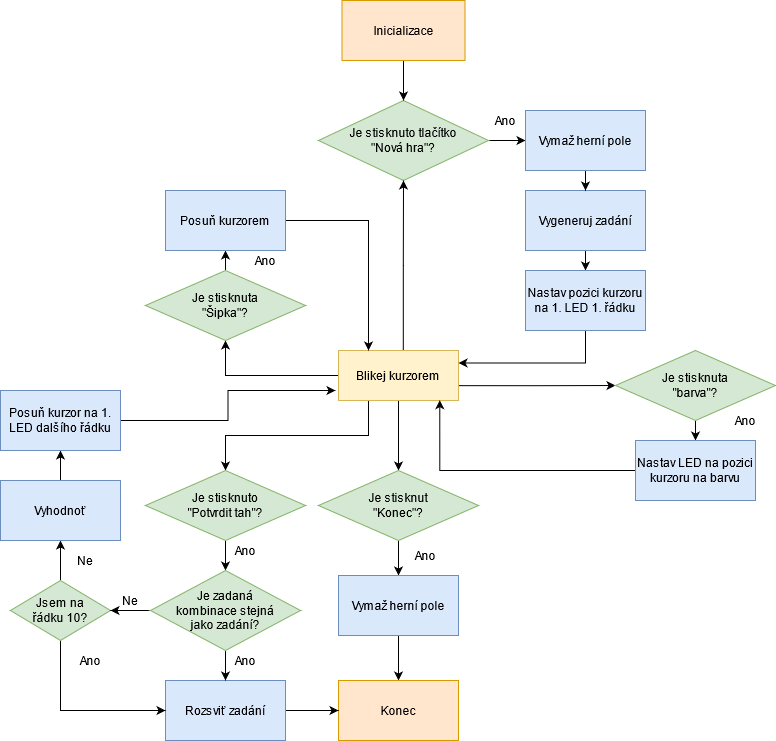
\includegraphics[scale=0.55]{obrazky/vyvojovy_diagram_1_hrac.png}
    \end{center}
    \caption[Vývojový diagram verze hry pro jednoho hráče]{Vývojový diagram verze hry pro jednoho hráče.}
    \end{figure}

\section{Hra pro dva hráče}
Varianta Elektronické hry Logic pro dva hráče má totožná pravidla s deskovou hrou. Po spuštění hry a stisku tlačítka "Nová hra"\ bliká 
kurzor v poli inteligentních LED se zadáním. První hráč zadává barvy pomocí barevných tlačítek a v poli LED se pohybuje pomocí šipek 
interpretovanými tlačítky. Hráč zadání zakryje stříškou a stiskne tlačítko „Potvrdit tah“. 

Po stisku zadání zůstane svítit a kurzor se přesune na první herní LED. Druhý hráč hledá zadanou kombinaci a tuto náhodnou kombinaci 
navolí pomocí barevných tlačítek. Kurzorem může taktéž pohybovat pomocí šipek interpretovanými tlačítky.
Pokud hráč zadá barvu, kterou zadat nechce, má dvě možnosti,
jak ji smazat. Kurzorem vybere danou barvu a buď ji hned změní na jinou barvu pomocí daného barevného tlačítka, nebo stiskne tlačítko 
stejné barvy a barva se smaže. Po zadání kombinace 
druhý hráč stiskne tlačítko „Potvrdit tah“\  a kurzor se přesune na první pozici vyhodnocovacího pole. 

První hráč má v tuto chvíli aktivní pouze šipky a červené a žluté barevné tlačítko. Červenou barvu zadává jako první a 
indikuje jí, že některá barva druhého hráče je obsažena v zadání, a to na totožné pozici. Poté zadává žlutou barvu, kterou 
udává, že některá z barev prvního hráče je obsažena v zadání, ale na jiné pozici, než kam ji druhý hráč umístil. Vyhodnocení 
hráč záměrně neumisťuje na pozice, kterých se hodnocení týká. Zpravidla se zleva umisťují nejdříve všechna červená a až poté 
všechna žlutá hodnocení. 

Po dokončení hodnocení první hráč stiskne tlačítko "Potvrdit tah"\  a kurzor se opět přesune na první pozici dalšího řádku herního pole. 
Hra dále pokračuje obdobným způsobem.
Pokud druhý hráč nalezne správnou kombinaci, pak první hráč odkryje zadání pro možnou kontrolu a hra je u konce. Pro možnost další 
hry stiskne jeden z hráčů tlačítko „Nová hra“. Celé herní, vyhodnocovací pole i pole se zadáním je smazáno a kurzor je znovu posunut 
na první pozici pole se zadáním. 

Přepínač SW13 slouží pro nastavení hry na 3 nebo 4 pole. Pokud hráči umístí přepínač do polohy ON, tak zvolí variantu hry na 4 pole. 
V poloze 1 zvolí variantu hry na 3 pole a omezí tím pohyb kurzoru pouze na 3 pole v každém řádku každé herní části. Poslední pozice
nikdy nesvítí a nikdy se také nehodnotí. 

Pozice přepínače SW14 se ve variantě hry pro dva hráče ignoruje. 

\begin{figure}[!h]
    \begin{center}
        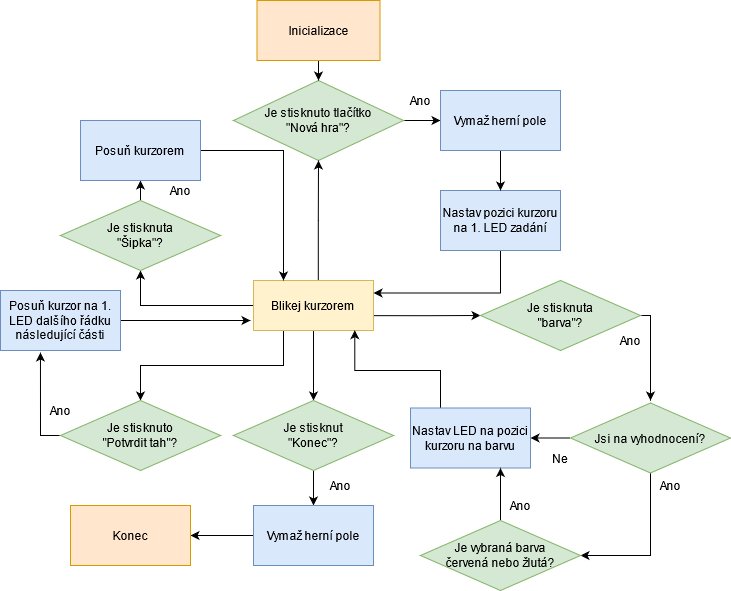
\includegraphics[scale=0.6]{obrazky/vyvojovy_diagram_2_hraci.png}
    \end{center}
    \caption[Vývojový diagram verze hry pro dva hráče]{Vývojový diagram verze hry pro dva hráče.}
    \end{figure}

\chapter{Krabička}
Krabička byla navržena v programu SolidWorks a vytištěna na 3D tiskárně. Spodní díl krabičky obsahuje 2 vyvýšené sloupky, ve kterých jsou otvory
na šrouby a matice. Vnitřní a nižší jsou určeny pro přišroubování DPS pomocí montážních otvorů a šroubů M3. Vnější otvory jsou poté pro přišroubování 
vrchního krytu krabičky. Otvor v horní části spodního dílu krabičky slouží pro umístění kolébkového vypínače. Na boční straně je také otvor
pro přivedení napájení USB konektorem.

Vrchní část krabičky obsahuje otvory pro LED a také pro tlačítka a přepínače. Tato část krabičky leží těsně nad DPS, aby nedocházelo k podsvitu LED přes
sebe a nemohlo tak docházet k podvodům během hry. 

Krabička také obsahuje tzv. stříšku, která je také součástí deskové hry. Tato stříška slouží pro zakrytí zadání ve hře pro dva hráče, kdy 
musí zadání svítit po celou dobu hry, aby byl druhý hráč schopen vyhodnocovat. Pro umístění stříšky slouží drážka ve vrchním dílu krabičky.

%obrázky

\chapter{Kompletace} 
Do spodního dílu krabičky byly do všech otvorů zalepeny matice M3 pomocí vteřinového lepidla. Do vrchního otvoru byl nasunut kolébkový vypínač, který
není třeba přilepit. Ke kolébkovému vypínači byly připájeny krátké drátové propojky.  

Do vnitřních otvorů byla přišroubována DPS pomocí šroubů M3$\times$6 se zápustnou hlavou. Klasické šrouby mají hlavičku, která je moc vysoká a krabička 
by nešla uzavřít. Zápustné šrouby jsou částečně zapuštěny do montážních otvorů DPS a tím je část hlavičky šroubu nad DPS nižší. 

Po uchycení DPS byly drátové prodlužky od kolébkového vypínače zasunuty do otvorů v DPS a připájeny.

Krabička byla následně přikryta vrchním dílem a přišroubována pomocí vnějších matic také šrouby M3$\times$6 se zápustnou hlavou. Ve vrchním dílu krabičky 
jsou otvory přizpůsobeny zápustným hlavám šroubů. Následně je možno zadání zakrýt stříškou, která se umisťuje do drážky ve vrchním dílu krabičky.
Po připojení jednoho z USB konektorů k napájecímu napětí je možno začít hrát.  
%obrázky

%%% Vložení souboru 'text/zaver' se závěrem
\chapter*{Závěr}
\phantomsection
\addcontentsline{toc}{chapter}{Závěr}

Byla navržena Elektronická hra Logic. Tato hra vychází ze stejnojmenné deskové hry.

V~této práci byla uvedena pravidla deskové hry Logic. Dále byl popsán kompletní návrh elektronické verze této hry. Při výběru elektronických 
komponent byl kladen důraz na spotřebu jednotlivých zařízení. Hru řídí mikrokontrolér ESP32-PICO. Herními prvky jsou inteligentní LED WS2812C, 
které jsou programovatelné a~jsou určeny pro přenosná zařízení. Hra Logic je integrována do jedné DPS, která řídí hru, a~zároveň jsou na této 
DPS umístěny herní prvky. Finální verze DPS obsahuje také měnič napětí, převodník z~USB na RS-232 a~převodníky úrovně. Napájení probíhá pomocí
USB konektorů.

Při návrhu je kladen velký důraz na vizuální podobu s~deskovou hrou Logic. Zároveň byla také zachována veškerá doporučená zapojení použitých 
čipů a~modulů a~rozmístění součástek na DPS.

V~neposlední řadě je stručně popsán vývoj od prvního prototypu až po finální verzi DPS. 

V~této práci je také popsáno softwarové řešení Elektronické hry Logic, včetně popisu funkce automatického vyhodnocení ve hře pro jednoho hráče.
Následuje popis ovládání Elektronické hry Logic, který je rozdělen na možnosti hry pro jednoho nebo pro dva hráče. 

Byla navržena a~vyrobena krabička. Tato krabička má všechny potřebné otvory a~DPS z~ní nemusí být nikdy vytahována. Obsahuje také stříšku pro
zakrytí zadání potřebnou ve hře pro dva hráče. 

%%% Vložení souboru 'text/literatura' se seznamem zdrojů
% Pro sazbu seznamu literatury použijte jednu z následujících možností

%%%%%%%%%%%%%%%%%%%%%%%%%%%%%%%%%%%%%%%%%%%%%%%%%%%%%%%%%%%%%%%%%%%%%%%%%
%1) Seznam citací definovaný přímo pomocí prostředí literatura / thebibliography

\begin{thebibliography}{99}

    \bibitem{Logic_pravidla}
    Klub deskových her Paluba:
    \emph{Logik pravidla}
    [cit.\,30.\,11.\,2020].
    Dostupné z URL:\\
    <\url{http://testapp.hrejsi.cz/logik/pravidla.htm}>.

\bibitem{WS2812C_datasheet}
    Worldsemi:
    \emph{WS2812C}
    Poslední aktualizace 06.\,12.\,2017 [cit.\,24.\,11.\,2020].
    Dostupné z URL:\\
    <\url{https://datasheet.lcsc.com/szlcsc/1810231210_Worldsemi-WS2812C_C114587.pdf}>.

\bibitem{Devkit_schema}
    Espressif:
    \emph{ESP32\_DevKic\_v4}
    Poslední aktualizace 06.\,12.\,2017 [cit.\,24.\,11.\,2020].
    Dostupné z URL:\\
    <\url{https://dl.espressif.com/dl/schematics/esp32_devkitc_v4-sch.pdf}>.

\bibitem{PICO_datasheet}
    Espressif Systems:
    \emph{ESP32-PICO-D4}
    Poslední aktualizace 2019 [cit.\,24.\,11.\,2020].
    Dostupné z URL:\\
    <\url{https://www.espressif.com/sites/default/files/documentation/esp32-pico-d4_datasheet_en.pdf}>.

\bibitem{JLCPCB}
    JLCPCB:
    \emph{JLCPCB}
    [cit.\,23.\,11.\,2020].
    Dostupné z URL:\\
    <\url{https://jlcpcb.com/}>.

\bibitem{JLCPCB_Capabilities}
    JLCPCB:
    \emph{PCB Capabilities}
    [cit.\,23.\,11.\,2020].
    Dostupné z URL:\\
    <\url{https://jlcpcb.com/capabilities/Capabilities}>.

\bibitem{SY8105_datasheet}
    SILERGY:
    \emph{Applocation Note:AN\_SY8105}
    [cit.\,24.\,11.\,2020].
    Dostupné z URL:\\
    <\url{https://datasheet.lcsc.com/szlcsc/Silergy-Corp-SY8105ADC_C178247.pdf}>.

\bibitem{CP2102_datasheet}
    Silicon Laboratories Inc.:
    \emph{CP2102N Data Sheet}
    USA: Poslední aktualizace květen 2016 [cit.\,24.\,11.\,2020].
    Dostupné z URL:\\
    <\url{https://www.silabs.com/documents/public/data-sheets/cp2102n-datasheet.pdf}>.

\end{thebibliography}


%%%%%%%%%%%%%%%%%%%%%%%%%%%%%%%%%%%%%%%%%%%%%%%%%%%%%%%%%%%%%%%%%%%%%%%%%
%%2) Seznam citací pomocí BibTeXu
%% Při použití je nutné v TeXnicCenter ve výstupním profilu aktivovat spouštění BibTeXu po překladu.
%% Definice stylu seznamu
%\bibliographystyle{unsrturl}
%% Pro českou sazbu lze použít styl czechiso.bst ze stránek
%% http://www.fit.vutbr.cz/~martinek/latex/czechiso.tar.gz
%%\bibliographystyle{czechiso}
%% Vložení souboru se seznamem citací
%\bibliography{text/literatura}
%
%% Následující příkaz je pouze pro ukázku sazby literatury při použití BibTeXu.
%% Způsobí citaci všech zdrojů v souboru odkazy.bib, i když nejsou citovány v textu.
%\nocite{*}

%%% Vložení souboru 'text/zkratky' se seznam použitých symbolů, veličin a zkratek
\cleardoublepage
\chapter*{\listofabbrevname}
\phantomsection
\addcontentsline{toc}{chapter}{\listofabbrevname}

\begin{acronym}[KolikMista]
%	\acro{A}
%		{Ampér (základní jednotka proudu)}
	\acro{Bd}
		{Baud - jednotka modulační rychlosti}
	\acro{C}
		{Kapacita}
	\acro{COM}
		{Common - sériový port RS-232}
	\acro{DPS}		
		{Deska plošného spoje}
	\acro{FDM}
		{Fused Deposition Modeling - technologie 3D tisku pomocí nanášení vrstev termoplastu}
	\acro{FLASH}
		{Typ paměti, která je trvalá - nesmaže se ani při ztrátě napájení}
	\acro{GND}
		{Ground - pin, který má nulový potenciál, vůči němu jsou referencované všechny ostatní signály}
	\acro{GPIO}
		{General Purpoise Input Output - piny, které mohou být vstupní nebo výstupní}
	\acro{kB}
		{Kilobajt - jednotka velikosti paměti}
%	\acro{}[k$\Omega$]
%		{Kiloohm (jednotka odporu)}	
	\acro{LDO}
		{Low-dropout regulator - regulátor napětí s nízkým úbytkem}
	\acro{LED}
		{Light-Emitting Diode - dioda emitující světlo}
	\acro{Li-Ion}
		{Lithium-iontový akumulátor - druh nabíjecí baterie}
%	\acro{mA}
%		{Miliampér (jednotka proudu)}
	\acro{mAh}
		{Miliampérhodina (jednotka kapacity používaná hlavně u~baterií)}
	\acro{MB}
		{Megabajt - jednotka velikosti paměti}
	\acro{MOSFET}
		{Metal Oxide Semiconductor Field Effect Transistor - tranzistor řízený elektrickým polem}	
	\acro{M3}
		{Metrický závit o~průměru 3~mm}
	\acro{RS-232}
		{Druh sériového komunikačního rozhraní} 
	\acro{RX}
		{Reciever - přijímač sériového rozhraní}
	\acro{SLA}
		{Stereolithography - technologie 3D tisku pomocí vytvrzování tekutého polymeru pomocí laserovéo záření}
	\acro{SMD}
		{Surface Mount Device - součástky určené pro povrchovou montáž} 
	\acro{SPI}
		{Serial peripheral interface - sériové periferní komunikační rozhraní}
	\acro{SRAM}
		{Static Random Acess Mamory - rychlá statické paměť, která se smaže při ztrátě napájení}	
	\acro{THT}
		{Through-hole technology - vývodová technologie součástek}
	\acro{TX}
		{Transciever - vysílač sériového rozhraní} 
	\acro{USB}
		{Universal Serial Bus - univerzální sériová sběrnice, která se používá pro připojení zařízení k~počítači}
%	\acro{V}
%		{Volt (základní jednotka napětí)}
	\acro{VDD}
		{Označení napájecího napětí}

\end{acronym}


%%% Vysázení seznamu obrázků
% (vynechejte, pokud máte dva nebo méně obrázků)
\listoffigures
\addcontentsline{toc}{chapter}{Seznam obrázků}

%%% Vysázení seznamu tabulek
% (vynechejte, pokud máte dvě nebo méně tabulek)
\listoftables
\addcontentsline{toc}{chapter}{Seznam tabulek}

%%% Vysázení seznamu výpisů kódu
% (vynechejte, pokud máte dva nebo méně výpisů)
\lstlistoflistings
\addcontentsline{toc}{chapter}{Seznam výpisů}

%%% Začátek příloh
\appendix

%%% Vysázení seznamu příloh
% (vynechejte, pokud máte dvě nebo méně příloh)
\listofappendices

%%% Vložení souboru 'text/prilohy' s přílohami
% Obvykle je přítomen alespoň popis co najdeme na přiloženém médiu
\chapter{Blokové schéma zapojení DPS finální verze}

\begin{figure}[!h]
    \begin{center}
      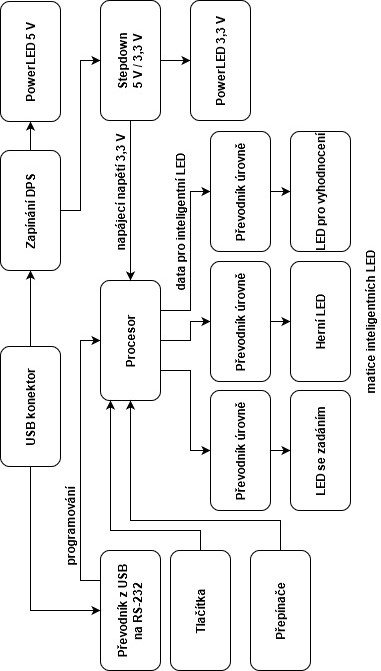
\includegraphics[scale=1.1]{prilohy/v2_blokove_schema.jpg}
    \end{center}
    \caption[Blokové schéma DPS finální verze]{Blokové schéma DPS finální verze.}
  \end{figure}

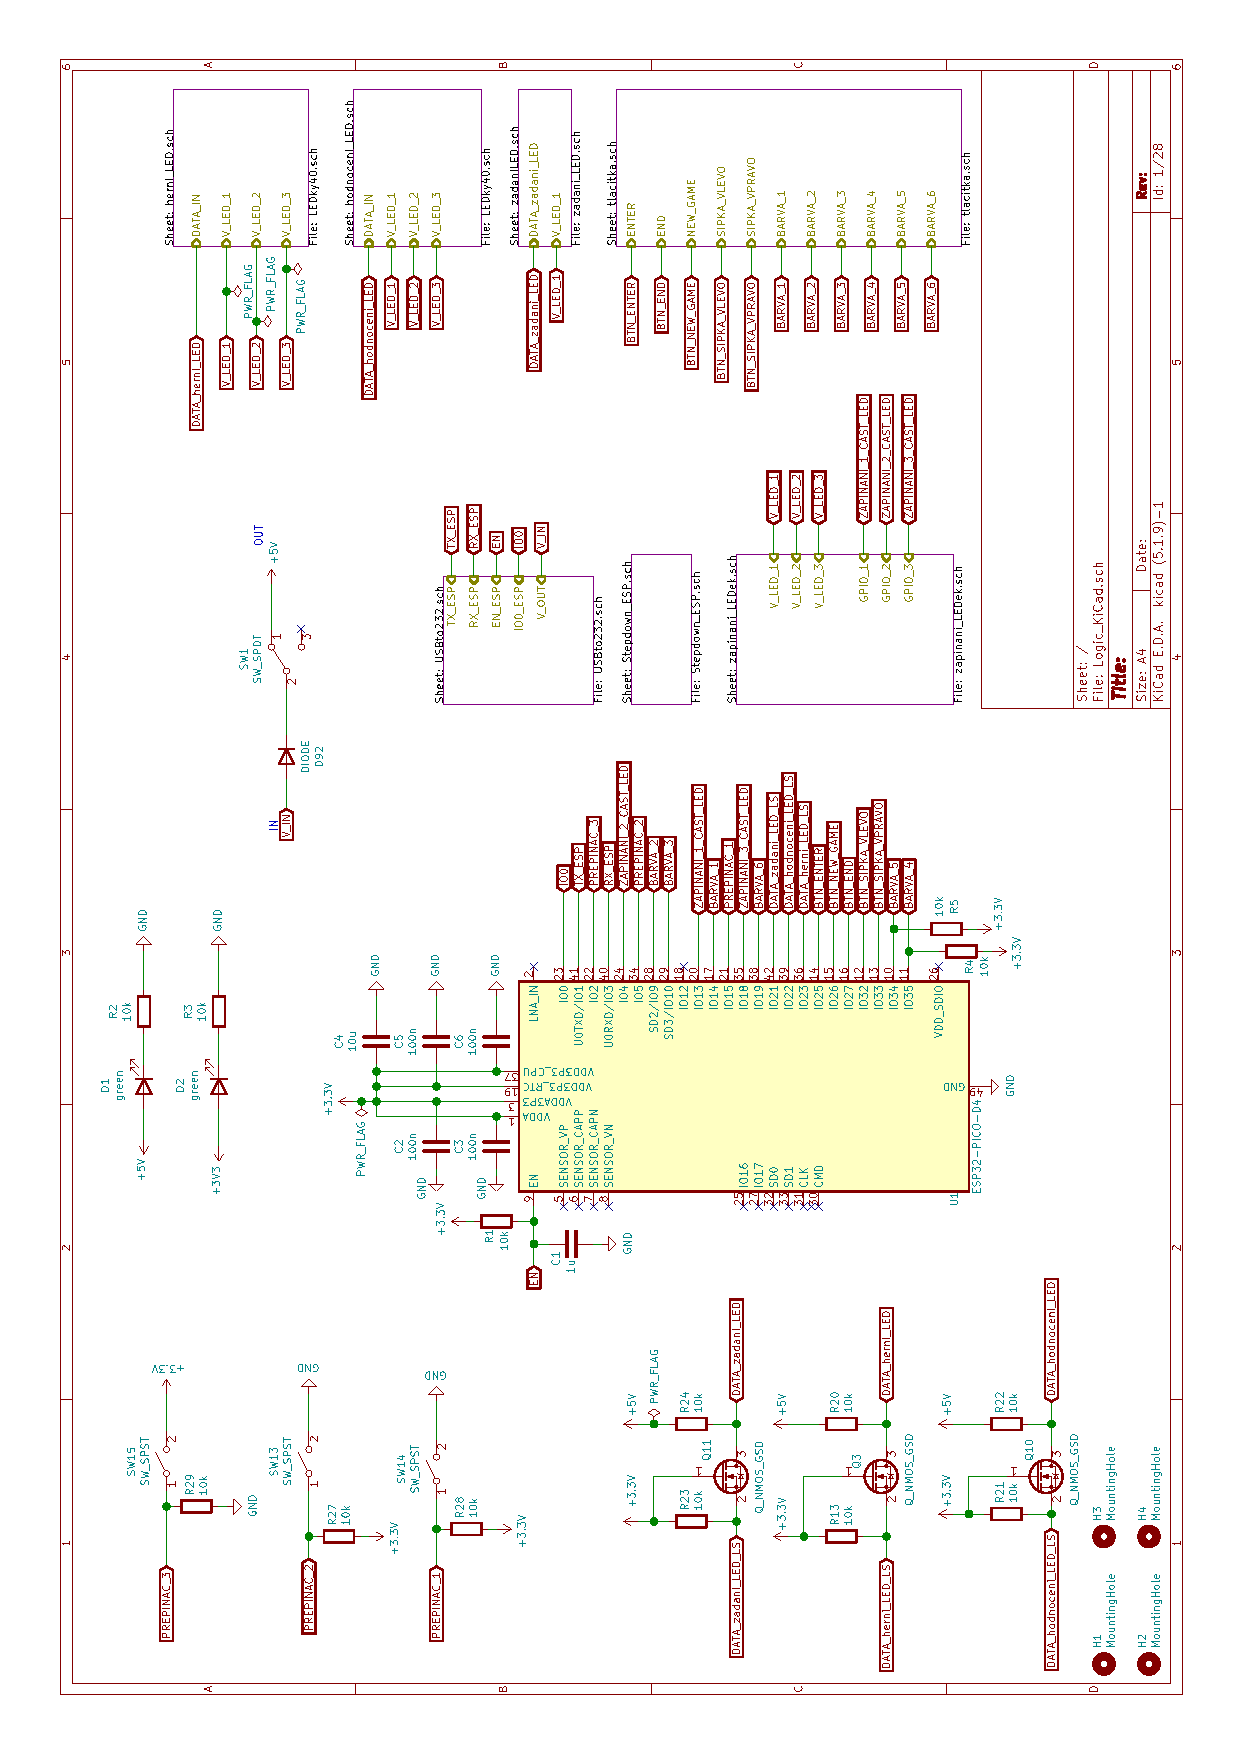
\includepdf[pages=1]{prilohy/cele}

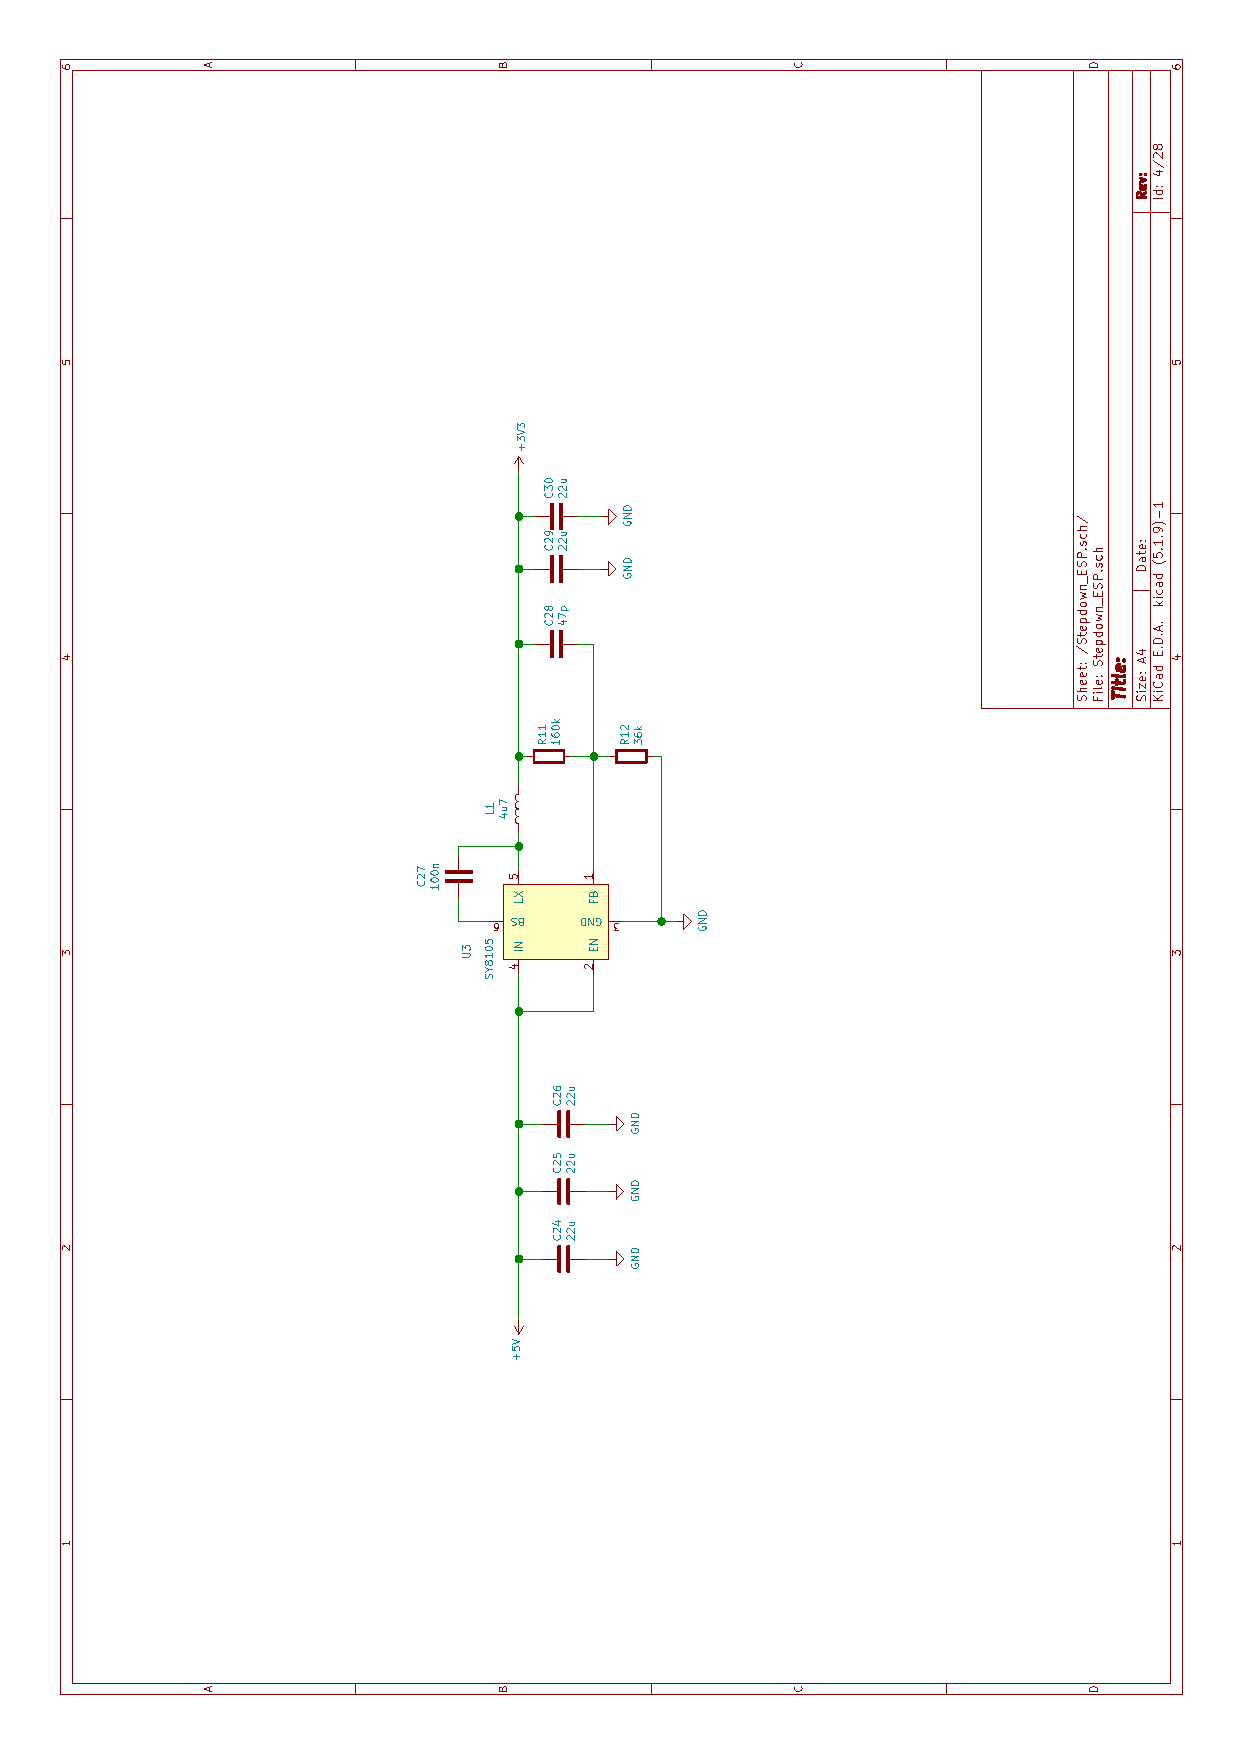
\includepdf[pages=1]{prilohy/Stepdown_ESP}

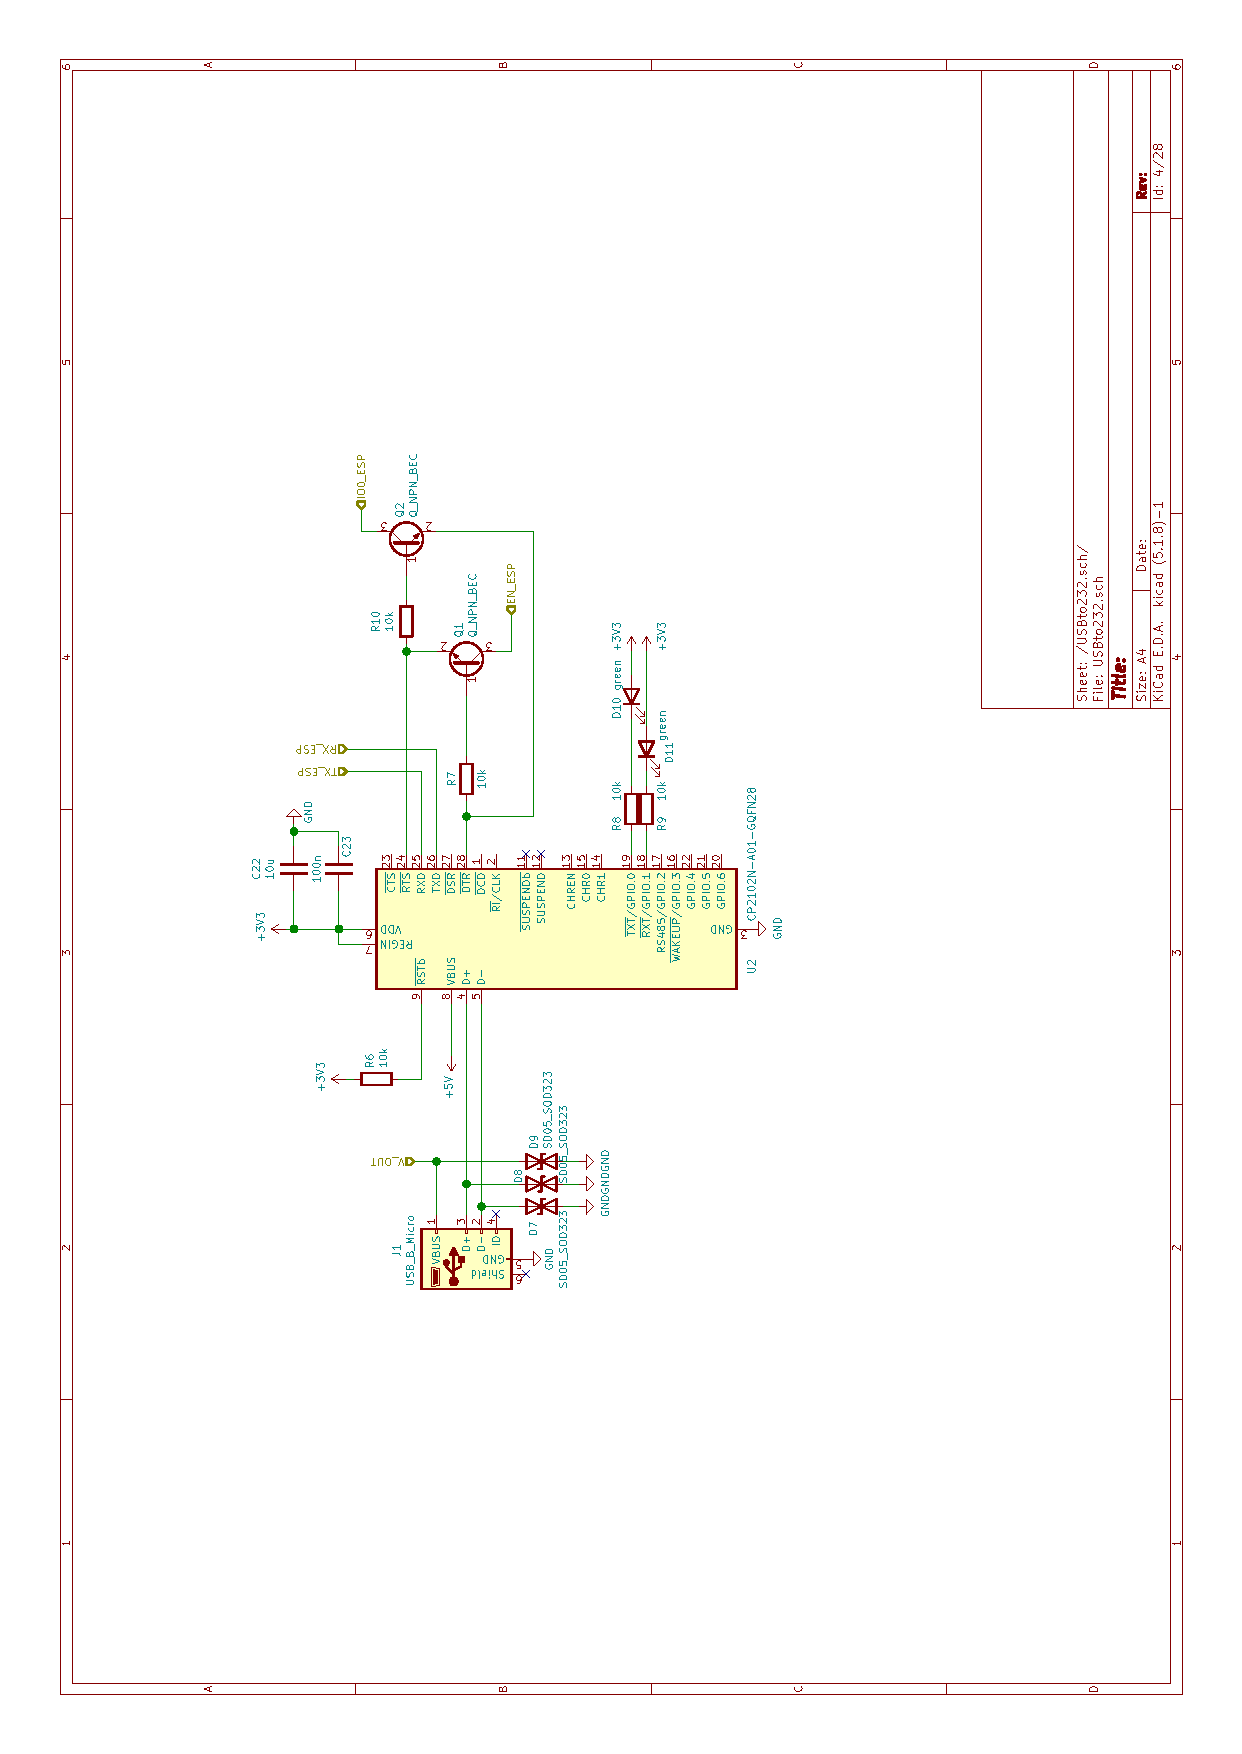
\includepdf[pages=1]{prilohy/USBto232}

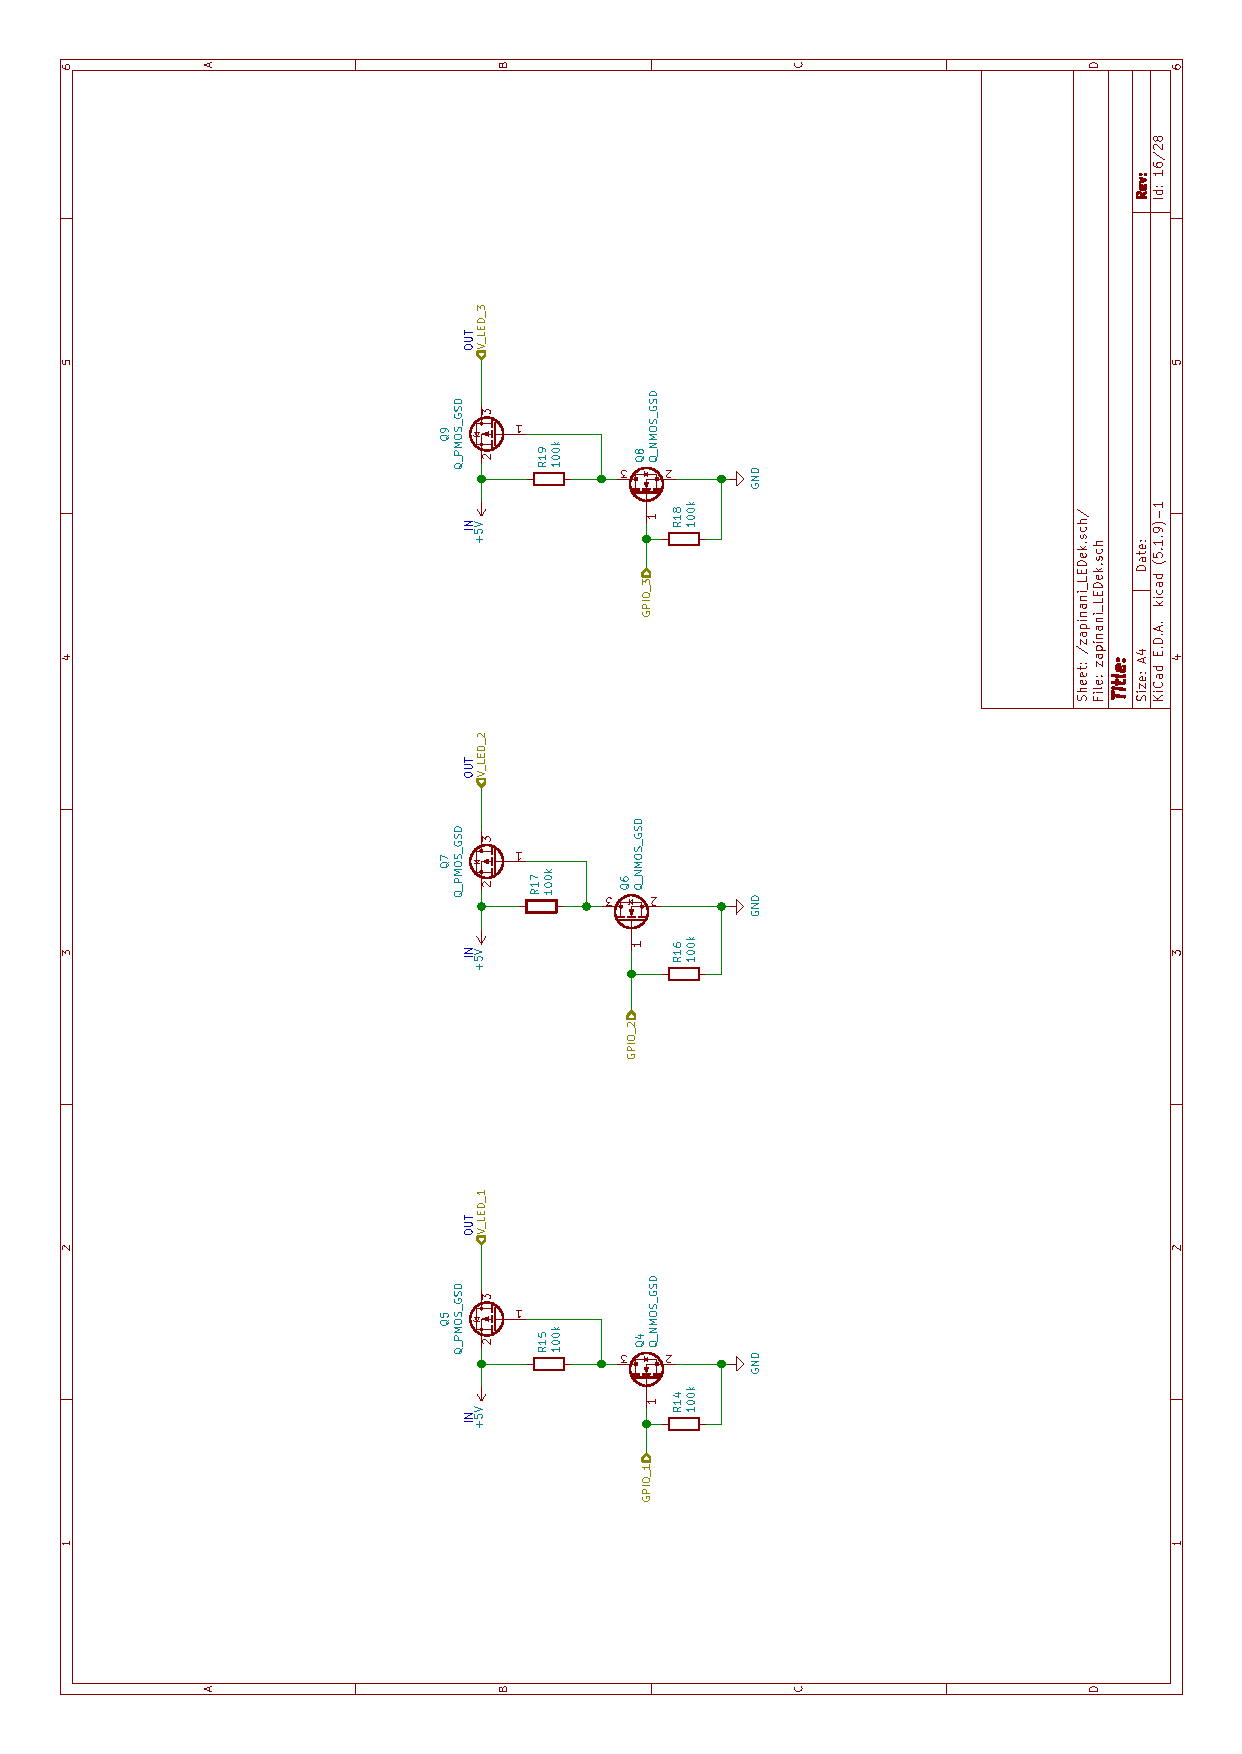
\includepdf[pages=1]{prilohy/zapinani_LEDek}

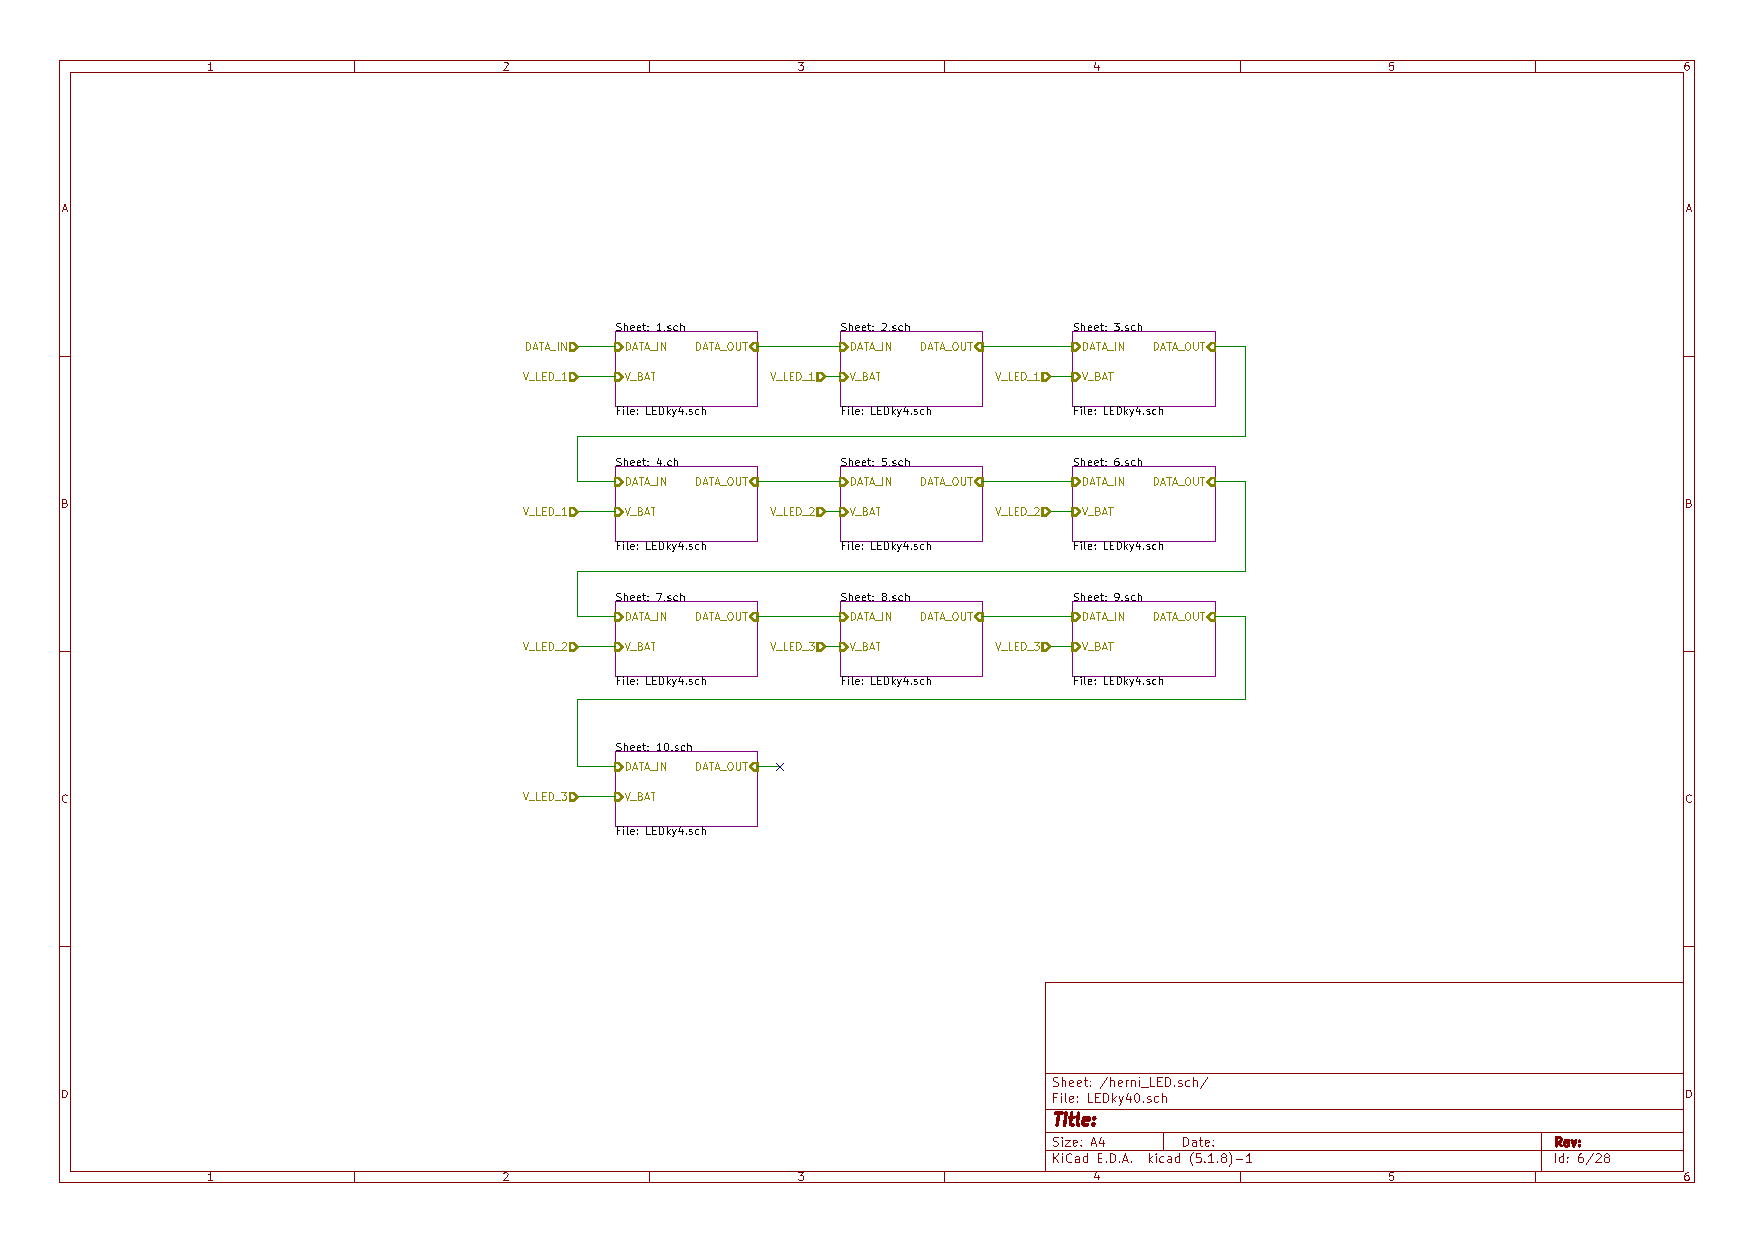
\includepdf[pages=1]{prilohy/LEDky40}

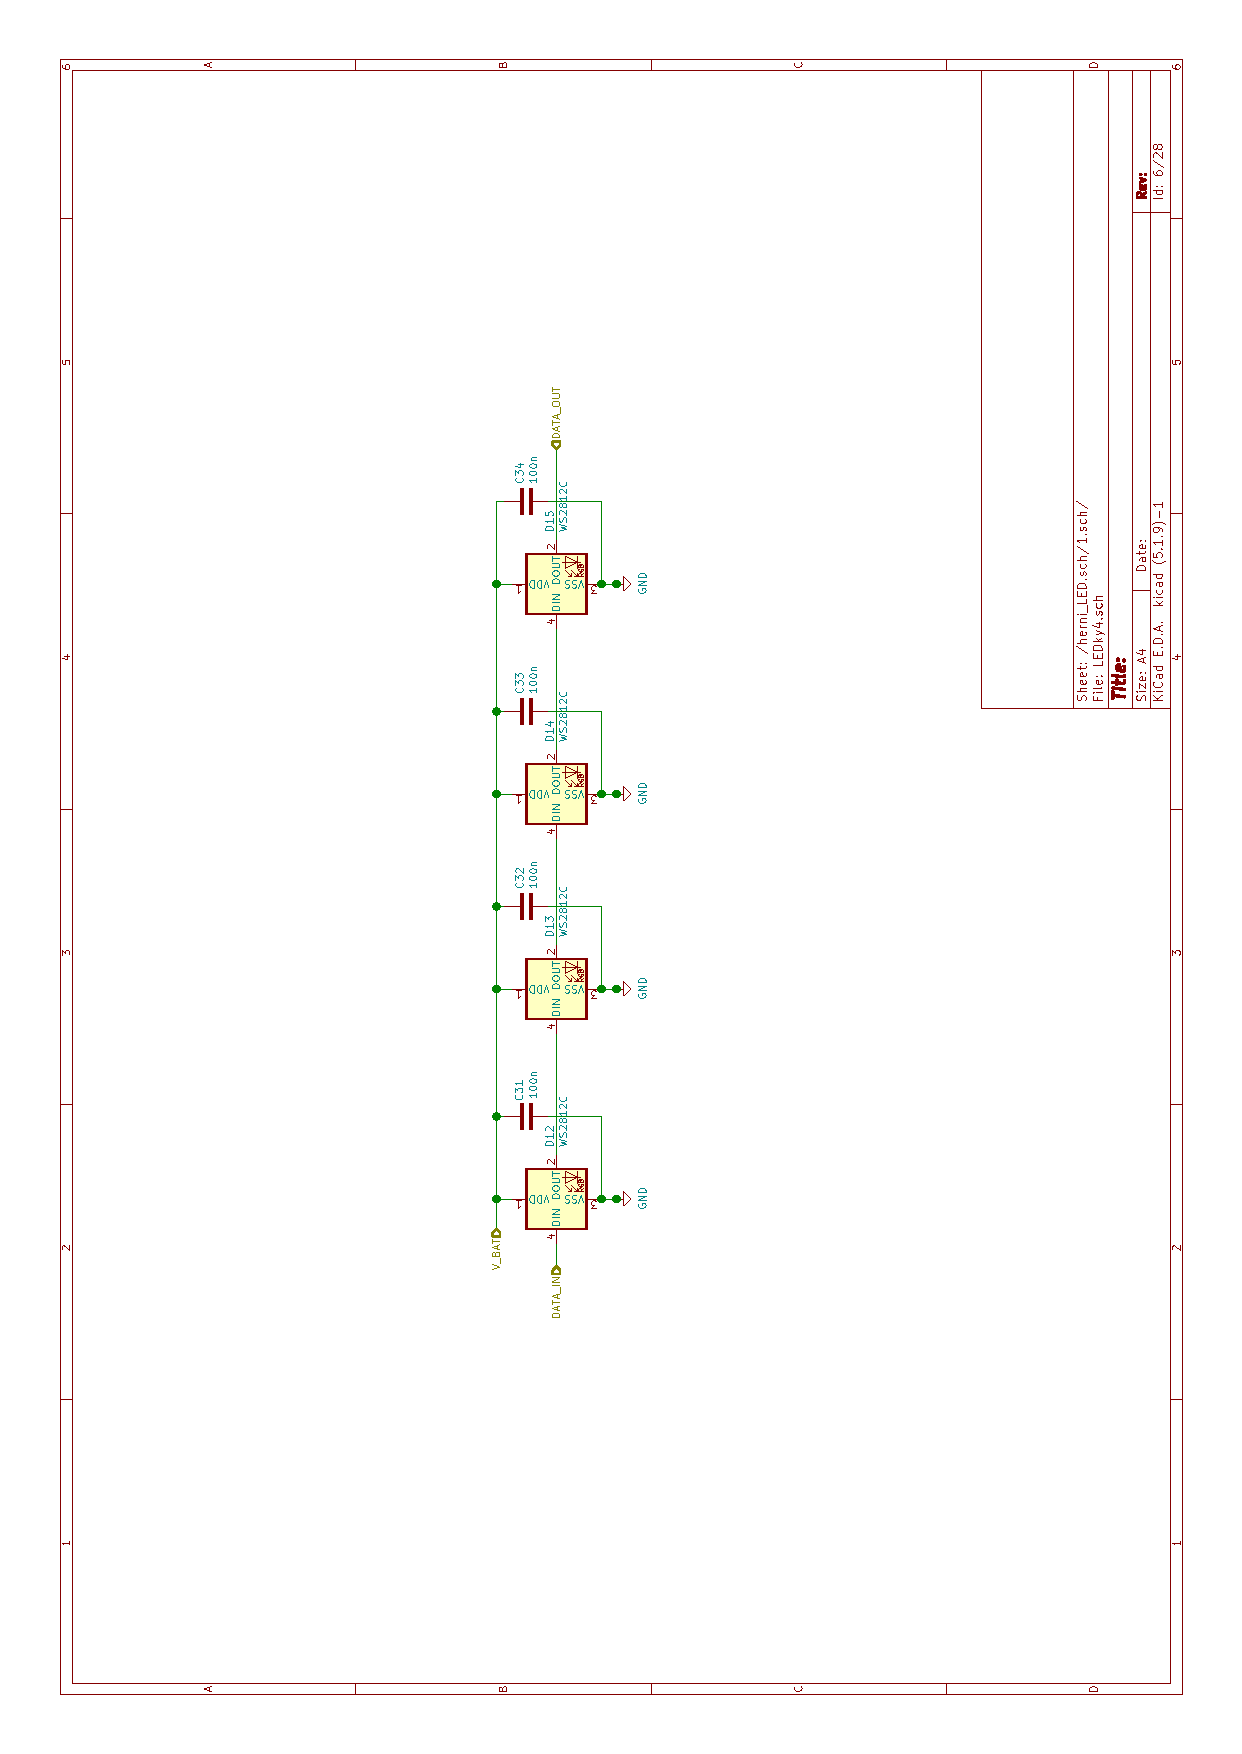
\includepdf[pages=1]{prilohy/LEDky4}

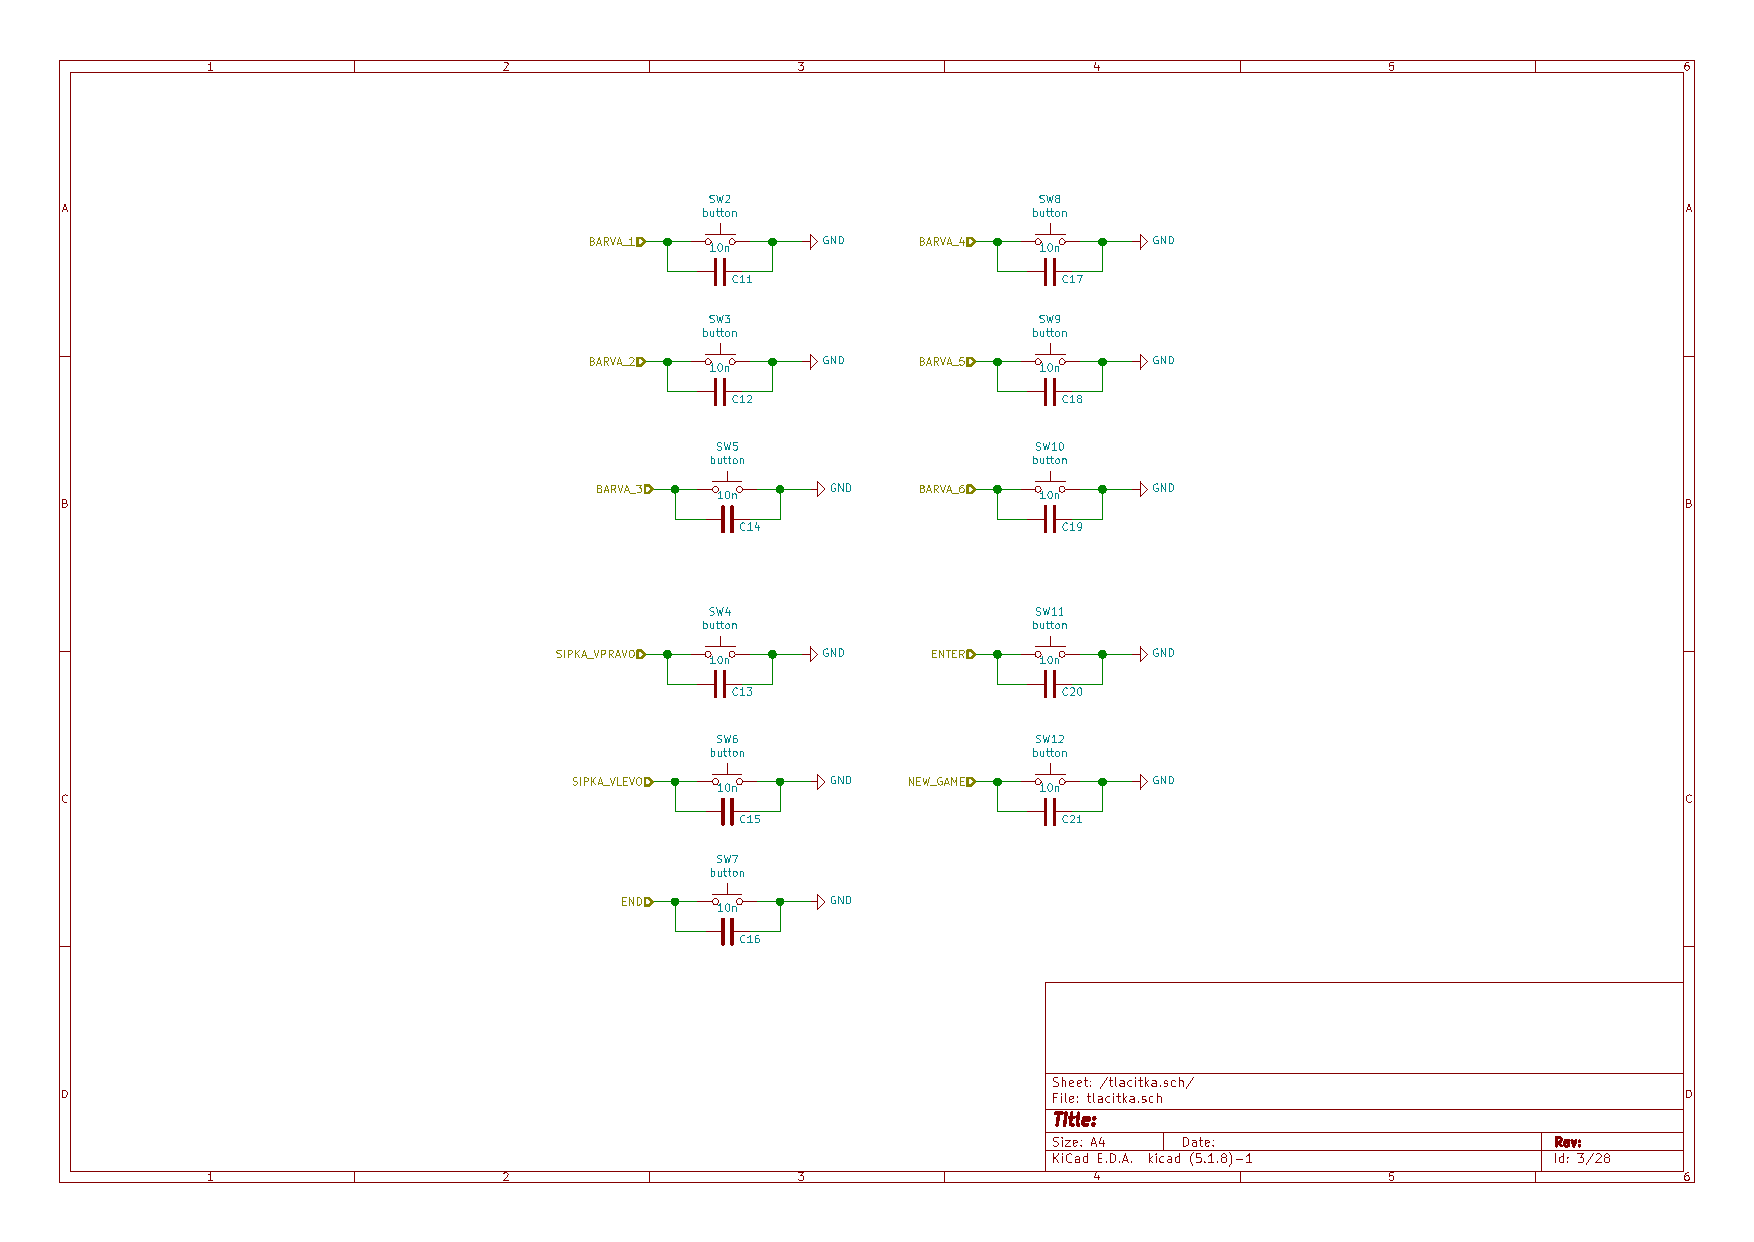
\includepdf[pages=1]{prilohy/tlacitka}

\chapter{Výrobní podklady DPS finální verze}

  \begin{figure}[!h]
    \begin{center}
      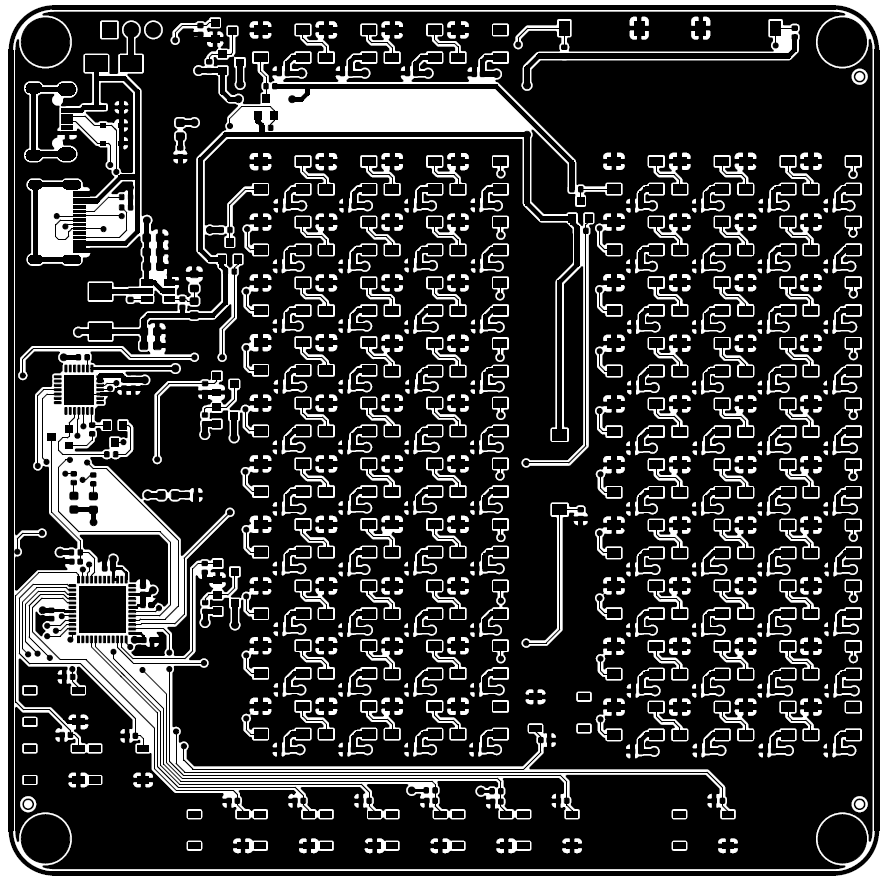
\includegraphics[scale=0.7]{prilohy/Verze2_vrstva_Cu_TOP.png}
    \end{center}
    \caption[Vrstva mědi TOP]{Vrstva mědi TOP.}
  \end{figure}

  \begin{figure}[!h]
    \begin{center}
      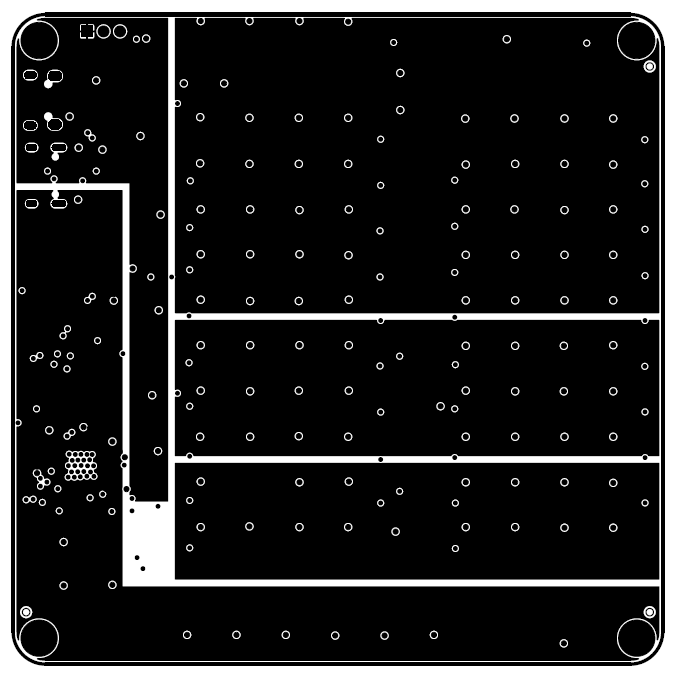
\includegraphics[scale=0.9]{prilohy/Verze2_vrstra_Cu_vnitrni_1.png}
    \end{center}
    \caption[Vnitří vrstva mědi napájení]{Vnitří vrstva mědi napájení.}
  \end{figure}

  \begin{figure}[!h]
    \begin{center}
      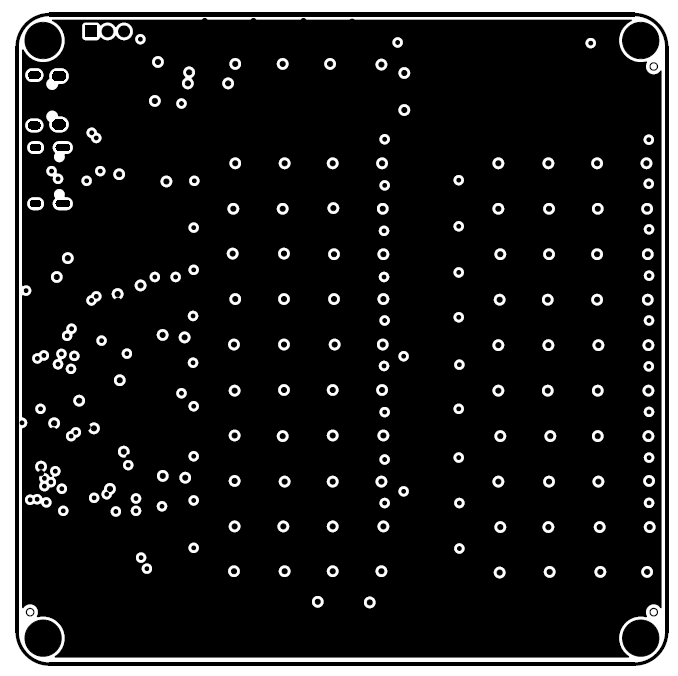
\includegraphics[scale=0.9]{prilohy/Verze2_vrstva_Cu_vnitrni_GND.png}
    \end{center}
    \caption[Vnitří vrstva mědi GND]{Vnitří vrstva mědi GND.}
  \end{figure}

  \begin{figure}[!h]
    \begin{center}
      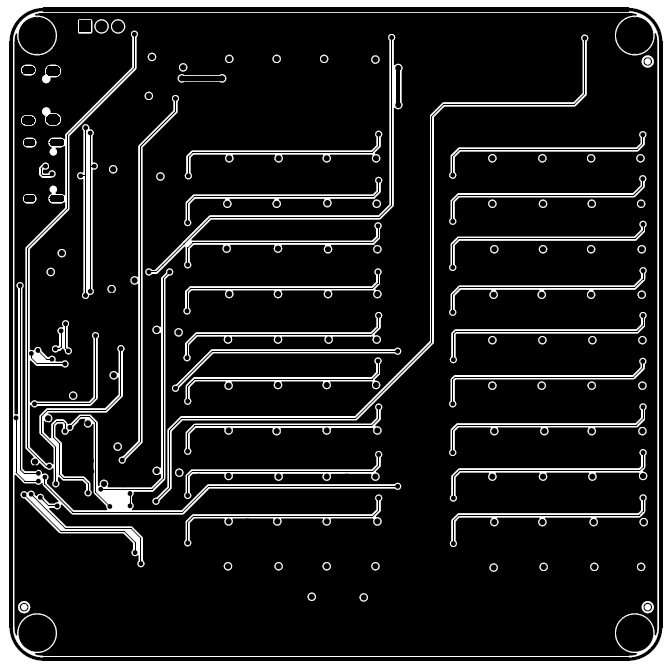
\includegraphics[scale=0.9]{prilohy/Verze2_vrstva_Cu_BOTTOM.png}
    \end{center}
    \caption[Vrstva mědi BOTTOM]{Vrstva mědi BOTTOM.}
  \end{figure}

  \begin{figure}[!h]
    \begin{center}
      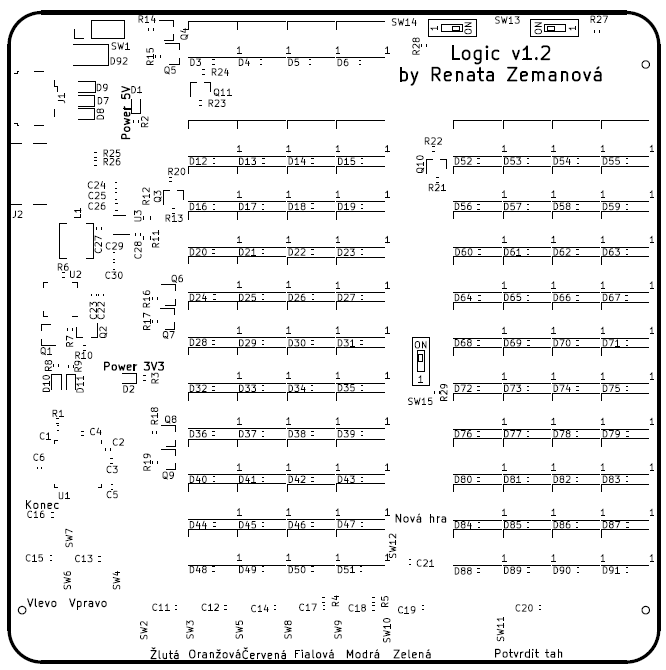
\includegraphics[scale=0.9]{prilohy/Verze2_vrstva_popisky_TOP.png}
    \end{center}
    \caption[Vrstva s~popisky TOP]{Vrstva s~popisky TOP.}
  \end{figure}

  \begin{figure}[!h]
    \begin{center}
      
\includegraphics[scale=0.9]{prilohy/Verze2_vrstva_popisky_BOTTOM.png}
    \end{center}
    \caption[Vrstva s~popisky BOTTOM]{Vrstva s~popisky BOTTOM.}
  \end{figure}

  \begin{figure}[!h]
    \begin{center}
      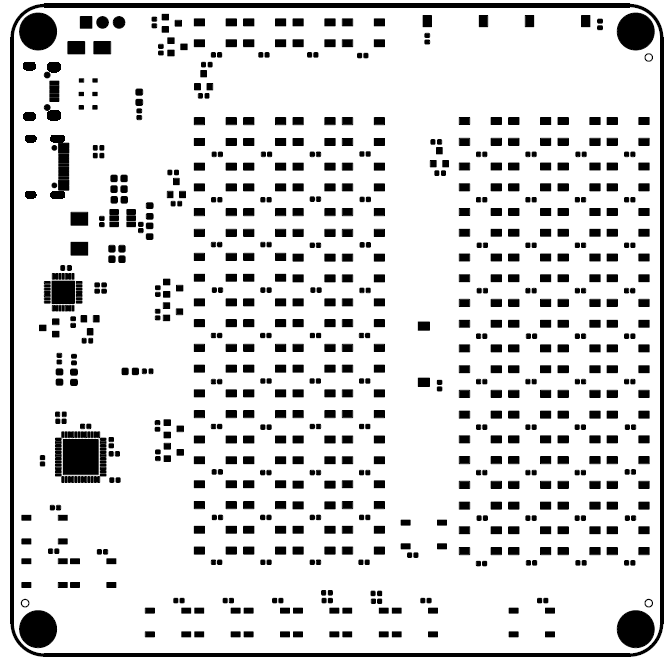
\includegraphics[scale=0.9]{prilohy/Verze2_maska_TOP.png}
    \end{center}
    \caption[Vrstva pro nanesení nepájivé masky TOP]{Vrstva pro nanesení nepájivé masky TOP.}
  \end{figure}

  \begin{figure}[!h]
    \begin{center}
      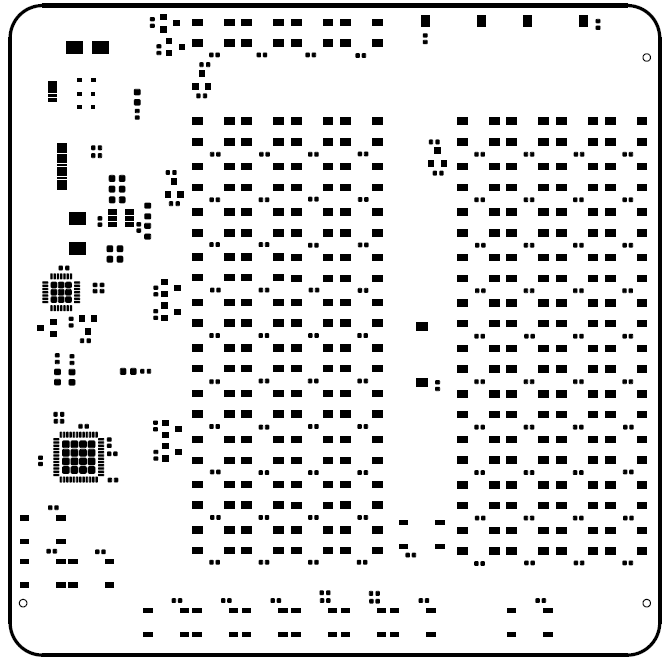
\includegraphics[scale=0.9]{prilohy/Verze2_pasta_TOP.png}
    \end{center}
    \caption[Vrstva pro nanesení pájecí pasty TOP]{Vrstva pro nanesení pájecí pasty TOP.}
  \end{figure}

  \begin{figure}[!h]
    \begin{center}
      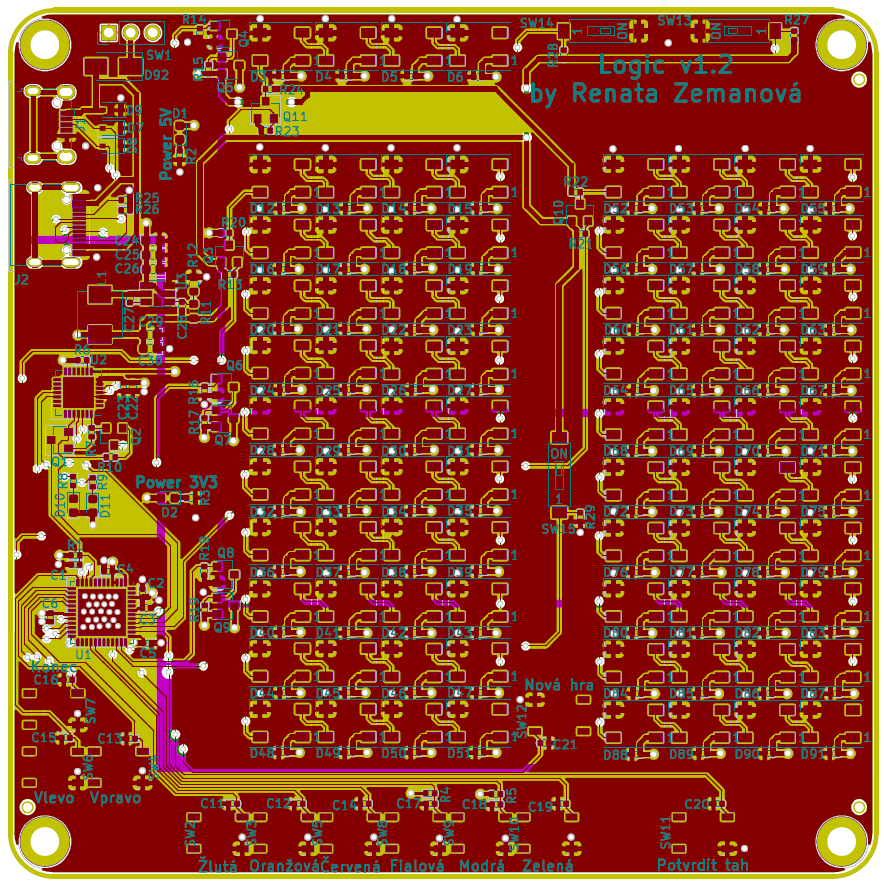
\includegraphics[scale=0.7]{prilohy/Verze2_DPS_cela.png}
    \end{center}
    \caption[Celá DPS]{Celá DPS.}
  \end{figure}

  %\chapter{Model krabičky}
  %krabička model SolidWorks


  %nejak to dostat na konec dokumentu!
  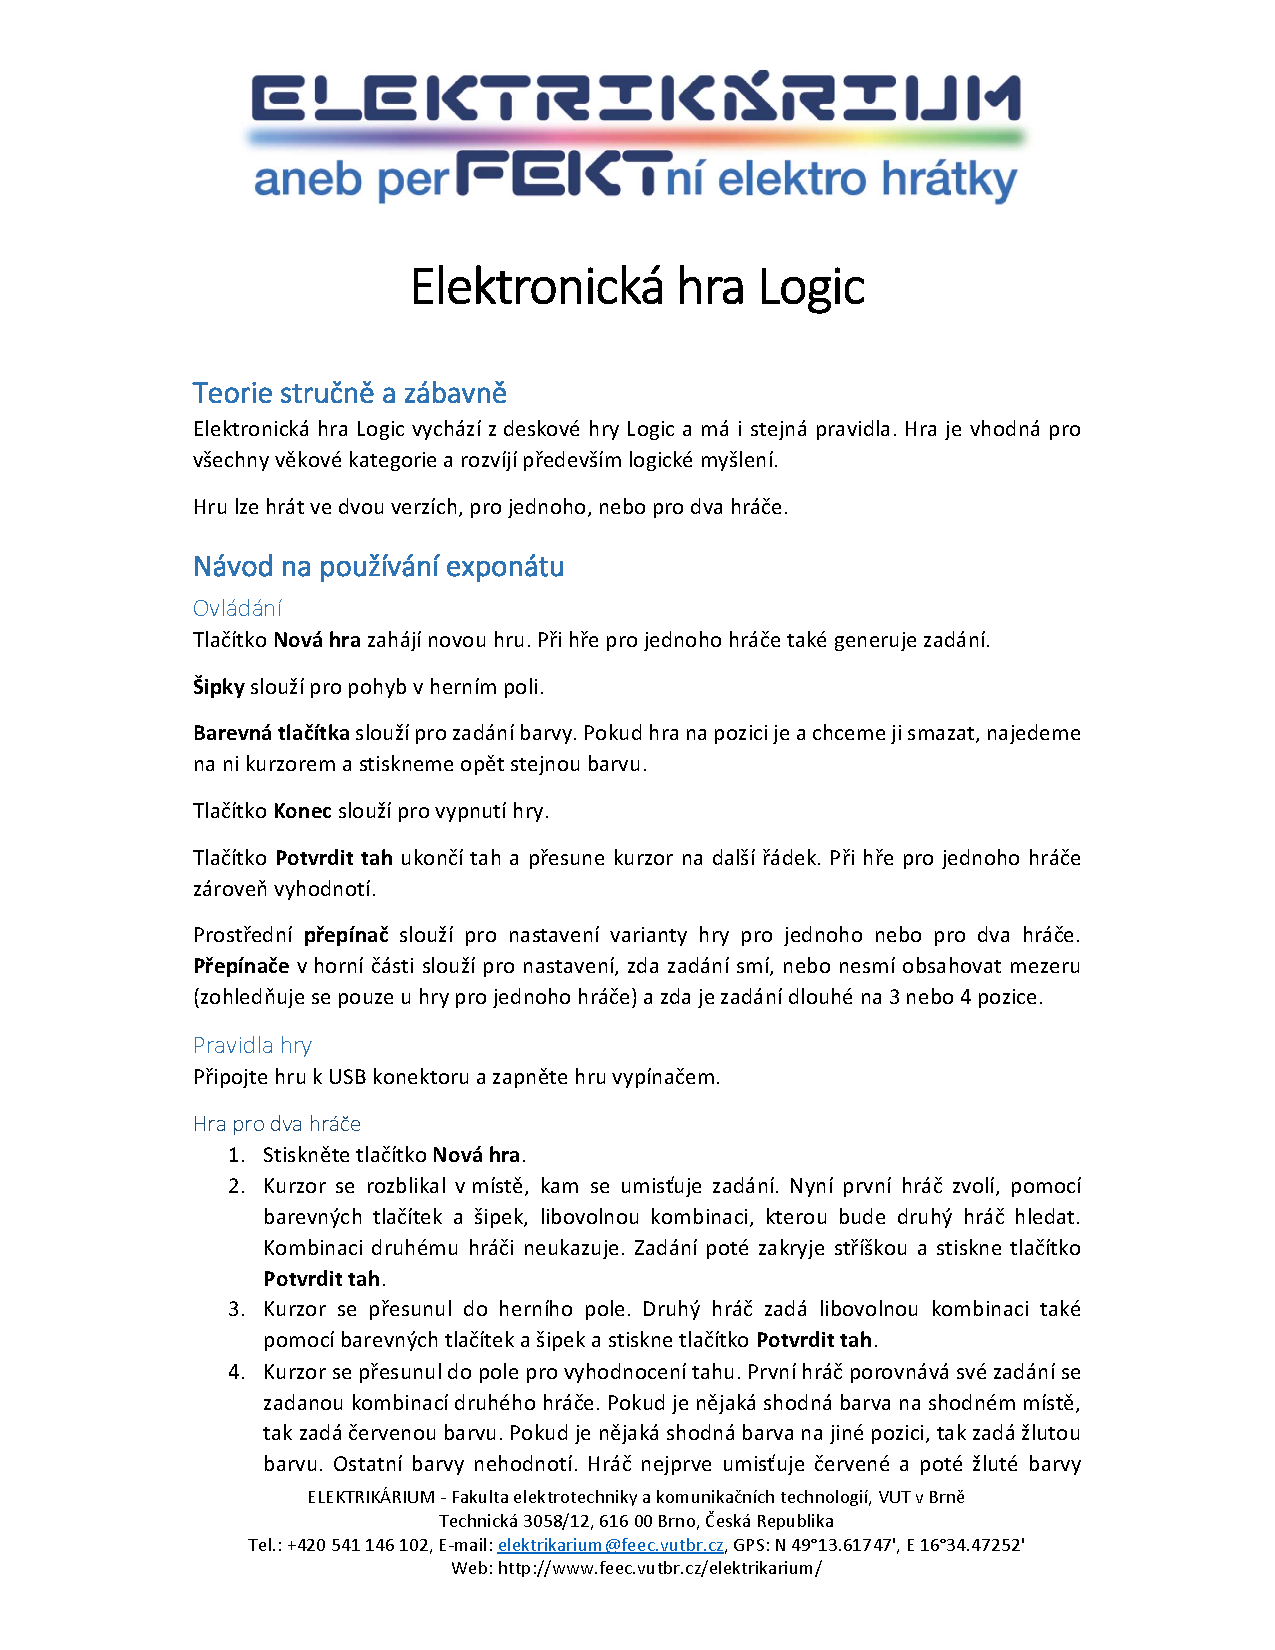
\includepdf[pages=1]{prilohy/Navod_Logic_Elektrikarium.pdf}

  \includepdf[pages=2]{prilohy/Navod_Logic_Elektrikarium.pdf}





\iffalse
\chapter{Některé příkazy balíčku \texttt{thesis}}

\section{Příkazy pro sazbu veličin a jednotek}

\begin{table}[!h]
  \caption[Přehled příkazů]{Přehled příkazů pro matematické prostředí }
  \begin{center}
  	\small
	  \begin{tabular}{|c|c|c|c|}
	    \hline
	    Příkaz    						& Příklad 					& Zdroj příkladu  							& Význam  \\
	    \hline\hline
	    \verb|\textind{...}|	& $\beta_\textind{max}$ 	& \verb|$\beta_\textind{max}$|	& textový index \\
	    \hline
	    \verb|\const{...}| 		& $\const{U}_\textind{in}$ 				& \verb|$\const{U}_\textind{in}$|		& konstantní veličina \\
	    \hline
	    \verb|\var{...}| 		& $\var{u}_\textind{in}$ & \verb|$\var{u}_\textind{in}$| & proměnná veličina \\
	    \hline
	    \verb|\complex{...}| 	& $\complex{u}_\textind{in}$ & \verb|$\complex{u}_\textind{in}$| & komplexní veličina \\
	    \hline
	    \verb|\vect{...}| 		& $\vect{y}$ 						& \verb|$\vect{y}$| & vektor \\
	    \hline
	    \verb|\mat{...}| 	& $\mat{Z}$ 						& \verb|$\mat{Z}$| & matice \\
	    \hline
	    \verb|\unit{...}| 		& $\unit{kV}$ 						& \verb|$\unit{kV}$|\quad či\ \, \verb|\unit{kV}| & jednotka \\
	    \hline
	  \end{tabular}
  \end{center}
\end{table}



%\newpage
\section{Příkazy pro sazbu symbolů}

\begin{itemize}
  \item
    \verb|\E|, \verb|\eul| -- sazba Eulerova čísla: $\eul$,
  \item
    \verb|\J|, \verb|\jmag|, \verb|\I|, \verb|\imag| -- sazba imaginární jednotky: $\jmag$, $\imag$,
  \item
    \verb|\dif| -- sazba diferenciálu: $\dif$,
  \item
    \verb|\sinc| -- sazba funkce: $\sinc$,
  \item
    \verb|\mikro| -- sazba symbolu mikro stojatým písmem%
			\footnote{znak pochází z~balíčku \texttt{textcomp}}: $\mikro$,
	\item
		\verb|\uppi| -- sazba symbolu $\uppi$
			(stojaté řecké pí, na rozdíl od \verb|\pi|, což sází $\pi$).
\end{itemize}
%
Všechny symboly jsou určeny pro matematický mód, vyjma \verb|\mikro|, jenž je\\ použitelný rovněž v~textovém módu.
%$\upmikro$


\chapter{Druhá příloha}

\begin{figure}[!h]
  \begin{center}
    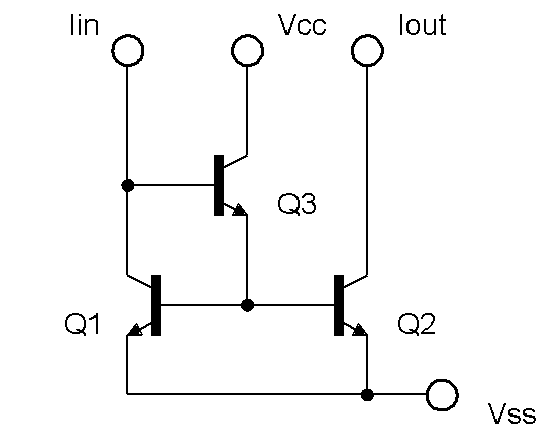
\includegraphics[scale=0.5]{obrazky/ZlepseneWilsonovoZrcadloNPN}
  \end{center}
  \caption[Alenčino zrcadlo]{Zlepšené Wilsonovo proudové zrcadlo.}
\end{figure}

Pro sazbu vektorových obrázků přímo v~\LaTeX{}u je možné doporučit balíček \href{https://www.ctan.org/pkg/pgf}{\texttt{TikZ}}.
Příklady sazby je možné najít na \href{http://www.texample.net/tikz/examples/}{\TeX{}ample}.
Pro vyzkoušení je možné použít programy QTikz nebo TikzEdt.




\chapter{Příklad sazby zdrojových kódů}

\section{Balíček \texttt{listings}}

Pro vysázení zdrojových souborů je možné použít balíček \href{https://www.ctan.org/pkg/listings}{\texttt{listings}}.
Balíček zavádí nové prostředí \texttt{lstlisting} pro sazbu zdrojových kódů, jako například:
%
\begin{lstlisting}[language={[LaTeX]TeX}]
\section{Balíček lstlistings}
Pro vysázení zdrojových souborů je možné použít
	balíček \href{https://www.ctan.org/pkg/listings}%
	{\texttt{listings}}.
Balíček zavádí nové prostředí \texttt{lstlisting} pro
	sazbu zdrojových kódů.
\end{lstlisting}
%
Podporuje množství programovacích jazyků.
Kód k~vysázení může být načítán přímo ze zdrojových souborů.
Umožňuje vkládat čísla řádků nebo vypisovat jen vybrané úseky kódu.
Např.:

\noindent
Zkratky jsou sázeny v~prostředí \texttt{acronym}:
\label{lst:zkratky}
\lstinputlisting[language={[LaTeX]TeX},nolol,numbers=left, firstnumber=6, firstline=6,lastline=6]{text/zkratky.tex}
%
Šířka textu volitelného parametru \verb|KolikMista| udává šířku prvního sloupce se zkratkami.
Proto by měla být zadávána nejdelší zkratka nebo symbol.
Příklad definice zkratky \acs{symfvz} je na výpisu \ref{lst:symfvz}.

\shorthandoff{-}
\lstinputlisting[language={[LaTeX]TeX},frame=single,caption={Ukázka sazby zkratek},label=lst:symfvz,numbers=left,linerange={bsymfvz-\%\%\%\ esymfvz},includerangemarker=false]{text/zkratky.tex}
\shorthandon{-}

\noindent
Ukončení seznamu je provedeno ukončením prostředí:
\lstinputlisting[language={[LaTeX]TeX},nolol,numbers=left,firstnumber=26,linerange=26]{text/zkratky.tex}

\vspace{\fill}

\noindent
{\bf Poznámka k~výpisům s~použitím volby jazyka \verb|czech| nebo \verb|slovak|:}\newline
Pokud Váš zdrojový kód obsahuje znak spojovníku \verb|-|, pak překlad může skončit chybou.
Ta je způsobená tím, že znak \verb|-| je v~českém nebo slovenském nastavení balíčku \verb|babel| tzv.\ aktivním znakem.
Přepněte znak \verb|-| na neaktivní příkazem \verb|\shorthandoff{-}| těsně před výpisem a hned za ním jej vraťte na aktivní příkazem \verb|\shorthandon{-}|.
Podobně jako to je ukázáno ve zdrojovém kódu šablony.


\clearpage

%\section{Výpis kódu prostředí Matlab}
Na výpisu \ref{lst:priklad.vypis.kodu.Matlab} naleznete příklad kódu pro Matlab, na výpisu \ref{lst:priklad.vypis.kodu.C} zase pro jazyk~C.

\lstnewenvironment{matlab}[1][]{%
\iflanguage{czech}{\shorthandoff{-}}{}%
\iflanguage{slovak}{\shorthandoff{-}}{}%
\lstset{language=Matlab,numbers=left,#1}%
}{%
\iflanguage{slovak}{\shorthandon{-}}{}%
\iflanguage{czech}{\shorthandon{-}}{}%
}

\begin{matlab}[frame=single,float=htbp,caption={Příklad Schur-Cohnova testu stability v~prostředí Matlab.},label=lst:priklad.vypis.kodu.Matlab,numberstyle=\scriptsize, numbersep=7pt]
%% Priklad testovani stability filtru

% koeficienty polynomu ve jmenovateli
a = [ 5, 11.2, 5.44, -0.384, -2.3552, -1.2288];
disp( 'Polynom:'); disp(poly2str( a, 'z'))

disp('Kontrola pomoci korenu polynomu:');
zx = roots( a);
if( all( abs( zx) < 1))
    disp('System je stabilni')
else
    disp('System je nestabilni nebo na mezi stability');
end

disp(' '); disp('Kontrola pomoci Schur-Cohn:');
ma = zeros( length(a)-1,length(a));
ma(1,:) = a/a(1);
for( k~= 1:length(a)-2)
    aa = ma(k,1:end-k+1);
    bb = fliplr( aa);
    ma(k+1,1:end-k+1) = (aa-aa(end)*bb)/(1-aa(end)^2);
end

if( all( abs( diag( ma.'))))
    disp('System je stabilni')
else
    disp('System je nestabilni nebo na mezi stability');
end
\end{matlab}

\noindent
\begin{minipage}{\linewidth}

\begin{lstlisting}[frame=single,numbers=right,caption={Funkce init v~jazyce C++.},label=lst:priklad.vypis.kodu.C,basicstyle=\ttfamily\small, keywordstyle=\color{black}\bfseries\underbar,]
void _init_ (){
  pinMode(LED_PIN_GAME, OUTPUT);
  pinMode(LED_PIN_TASK, OUTPUT);
  pinMode(LED_PIN_EVAL, OUTPUT);

  pinMode(SET_POWER_LEDS_1_TO_4, OUTPUT);
  pinMode(SET_POWER_LEDS_5_TO_7, OUTPUT);
  pinMode(SET_POWER_LEDS_8_TO_10, OUTPUT);

  pinMode(SW_ENTER, INPUT_PULLUP);
  pinMode(SW_RIGHT, INPUT_PULLUP);
  pinMode(SW_LEFT, INPUT_PULLUP);
  pinMode(SW_END, INPUT_PULLUP);
  pinMode(SW_NEW_GAME, INPUT_PULLUP);
  pinMode(SW_YELLOW, INPUT_PULLUP);
  pinMode(SW_ORANGE, INPUT_PULLUP);
  pinMode(SW_RED, INPUT_PULLUP);
  pinMode(SW_PURPLE, INPUT_PULLUP);
  pinMode(SW_BLUE, INPUT_PULLUP);
  pinMode(SW_GREEN, INPUT_PULLUP);

  digitalWrite(SET_POWER_LEDS_1_TO_4, POWER_ON); 
  digitalWrite(SET_POWER_LEDS_5_TO_7, POWER_OFF);
  digitalWrite(SET_POWER_LEDS_8_TO_10, POWER_OFF);
}
\end{lstlisting}
\end{minipage}







\chapter{Obsah elektronické přílohy}
Elektronická příloha je často nedílnou součástí semestrální nebo závěrečné práce.
Vkládá se do informačního systému VUT v~Brně ve vhodném formátu (ZIP, PDF\,\dots).

Nezapomeňte uvést, co čtenář v~této příloze najde.
Je vhodné okomentovat obsah každého adresáře, specifikovat, který soubor obsahuje důležitá nastavení, který soubor je určen ke spuštění, uvést nastavení kompilátoru atd.
Také je dobře napsat, v~jaké verzi software byl kód testován (např.\ Matlab 2018b).
Pokud bylo cílem práce vytvořit hardwarové zařízení,
musí elektronická příloha obsahovat veškeré podklady pro výrobu (např.\ soubory s~návrhem DPS v~Eagle).

Pokud je souborů hodně a jsou organizovány ve více složkách, je možné pro výpis adresářové struktury použít balíček \href{https://www.ctan.org/pkg/dirtree}{\texttt{dirtree}}.

\bigskip

{\small
%
\dirtree{%.
.1 /\DTcomment{kořenový adresář přiloženého archivu}.
.2 logo\DTcomment{loga školy a fakulty}.
.3 BUT\_abbreviation\_color\_PANTONE\_EN.pdf.
.3 BUT\_color\_PANTONE\_EN.pdf.
.3 FEEC\_abbreviation\_color\_PANTONE\_EN.pdf.
.3 FEKT\_zkratka\_barevne\_PANTONE\_CZ.pdf.
.3 UTKO\_color\_PANTONE\_CZ.pdf.
.3 UTKO\_color\_PANTONE\_EN.pdf.
.3 VUT\_barevne\_PANTONE\_CZ.pdf.
.3 VUT\_symbol\_barevne\_PANTONE\_CZ.pdf.
.3 VUT\_zkratka\_barevne\_PANTONE\_CZ.pdf.
.2 obrazky\DTcomment{ostatní obrázky}.
.3 soucastky.png.
.3 spoje.png.
.3 ZlepseneWilsonovoZrcadloNPN.png.
.3 ZlepseneWilsonovoZrcadloPNP.png.
.2 pdf\DTcomment{pdf stránky generované informačním systémem}.
.3 student-desky.pdf.
.3 student-titulka.pdf.
.3 student-zadani.pdf.
.2 text\DTcomment{zdrojové textové soubory}.
.3 literatura.tex.
.3 prilohy.tex.
.3 reseni.tex.
.3 uvod.tex.
.3 vysledky.tex.
.3 zaver.tex.
.3 zkratky.tex.
%.2 navod-sablona\_FEKT.pdf\DTcomment{návod na používání šablony}.
.2 sablona-obhaj.tex\DTcomment{hlavní soubor pro sazbu prezentace k~obhajobě}.
%.2 readme.txt\DTcomment{soubor s~popisem obsahu CD}.
.2 sablona-prace.tex\DTcomment{hlavní soubor pro sazbu kvalifikační práce}.
.2 thesis.sty\DTcomment{balíček pro sazbu kvalifikačních prací}.
}
}
\fi

\end{document}